\documentclass{article}
\usepackage[utf8]{inputenc}
\usepackage{hyperref}
\usepackage{graphicx}
\usepackage[backend=bibtex]{biblatex}
\bibliography{main.bib}

\newcommand{\baseimagedir}{..}

\title{BeeGFS}
\author{Parsa Mohammadian\\ Arshia Akhavan}
\date{\today}

\begin{document}

\maketitle

\tableofcontents

\section{Introduction}
BeeGFS was developed at the Fraunhofer Institute for industrial mathematics (ITWM). It was originally released as “FhGFS”, but was newly labeled as BeeGFS (registered trade mark) in 2014. The formerly known FhGFS can still be found in some scripts or code. \cite{heichler2014introduction}

The decision to develop a new parallel file system was made in 2005 – and it was launched as a research project. The original motivation was born out of experiencing that available products neither scale the way users expect it – nor were they as easy to use and maintain as system administrators demand it. \cite{heichler2014introduction}

The first productive installation within the Fraunhofer Institute was made in 2007. It became very soon clear that the file system quickly evolved to a state which made it useful for HPC users. The first performing installation outside Fraunhofer followed in 2009. \cite{heichler2014introduction}

Since then the file system became increasingly popular in Europe and the US for being used in small, medium and large HPC systems. According to the number of installations BeeGFS is very much accepted and appreciated in academia – but also commercial customers do trust the product, too. \cite{heichler2014introduction}

\section{Background}

\section{Related Work}

\section{System}
\subsection{Overview}

\subsection{Design}
Our system design consists of 4 nodes, each with 4 Core of CPU and 8 Giga Bytes of RAM as shown in Figure \ref{fig:overal-system-design}. The CPU used in this Experiment is Intel's Xeon Bronze 3106 Processor. Each node has 150 Giga Bytes of SSD mounted as /dev/sda. Ubuntu 20.04 is installed on all of the nodes. 

\begin{figure}
    \centering
    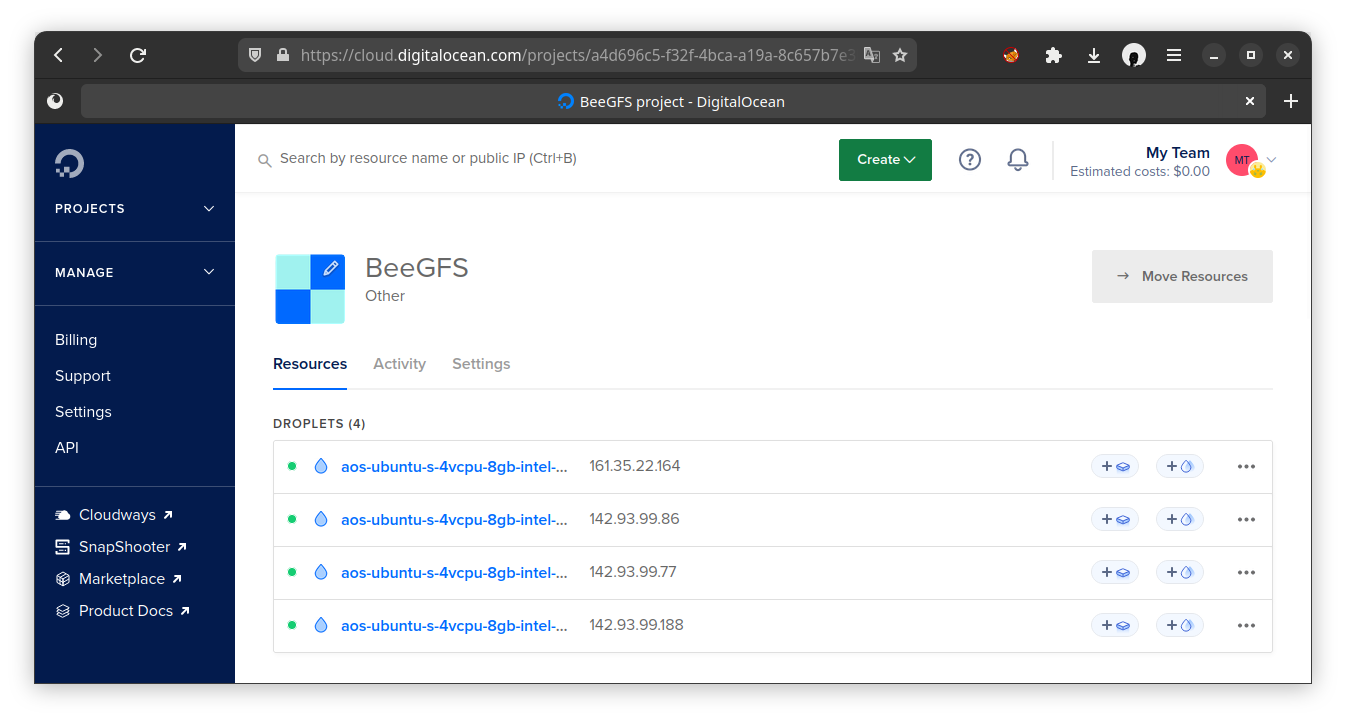
\includegraphics[width=0.45\linewidth]{\baseimagedir/misc/do-project.png}
    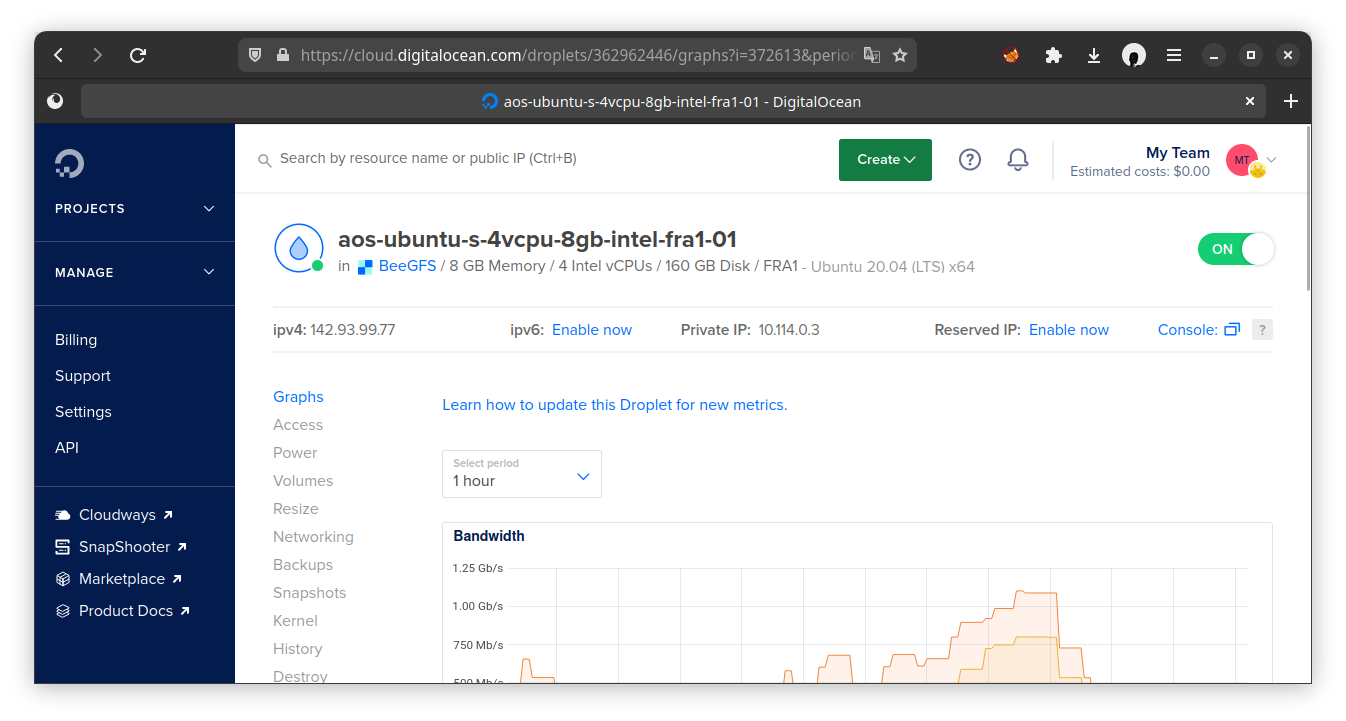
\includegraphics[width=0.45\linewidth]{\baseimagedir/misc/do-droplet.png}
    \caption{Overall system design}
    \label{fig:overal-system-design}
\end{figure}

The file system is deployed on two nodes. management and metadata server are both deployed on the same node. Each node consist of one storage server (total of two storage servers each with 150GB capacity).

The other two nodes are used as BeeGFS clients and are configured for benchmarking.


\subsection{Implementation}
BeeGFS Server are installed using docker containers provided by BeeGFS itself. The directories for storage servers are mounted to bypass OverlayFS overhead for IO intensive workloads.
BeeGFS clients are installed and executed using systemd. A BeeGFS kernel module is installed to further optimized the use of BeeGFS mounted filesystem.

both BeeGFS server and client are deployed using Ansible and can be seen \hyperlink{https://github.com/Parsa2820/BeeGFS-Benchmark/tree/master/ansible}{here}
We developed an Ansible-galaxy role for installing BeeGFS servers using Docker and extended an already provided ansible-galaxy role for deploying BeeGFS clients. 
\section{Evaluation}
In order to evaluate the performance of BeeGFS, we have used the IOZone benchmark.
IOZone is a filesystem benchmark tool. The benchmark generates and measures 13 types of file operations which are listed below: \cite{iozoneexample}
\begin{itemize}
    \item Read - Indicates the performance of reading a file that already exists in the filesystem.
    \item Write - Indicates the performance of writing a new file to the filesystem.
    \item Re-read - After reading a file, this indicates the performance of reading a file again.
    \item Re-write - Indicates the performance of writing to an existing file.
    \item Random Read - Indicates the performance of reading a file by reading random information from the file. i.e this is not a sequential read.
    \item Random Write - Indicates the performance of writing to a file in various random locations. i.e this is not a sequential write.
    \item Backward Read
    \item Record Re-Write
    \item Stride Read
    \item Fread
    \item Fwrite
    \item Freread
    \item Frewrite
\end{itemize}
The IOZone benchmark script can be found in the \texttt{benchmark/IOZone.sh \footnote{\url{https://github.com/Parsa2820/BeeGFS-Benchmark/blob/master/benchmark/IOZone.sh}}} file. The script is written in bash and it takes the following arguments:
\begin{itemize}
    \item Directory in which to run IOZone (should be a BeeGFS mount point)
    \item Output log file name
    \item File size (in IOZone recognized units)
\end{itemize}
The script runs IOZone with the passed arguments and saves the standard output in the specified log file. Another file is created within the specified directory which contains benchmark results in Excel format. The latter file then is parsed by the \texttt{result/excel-to-chart.ipynb \footnote{\url{https://github.com/Parsa2820/BeeGFS-Benchmark/blob/master/result/excel-to-chart.ipynb}}} Jupyter notebook and the results are plotted in a chart. The charts are accessible both in the notebook and in the \texttt{result/excel-to-chart \footnote{\url{https://github.com/Parsa2820/BeeGFS-Benchmark/tree/master/result/excel-to-chart}}} directory.

The initial benchmark was run on a single BeeGFS client node which had a single node BeeGFS cluster mounted on it. The benchmark was run on 1MB, 10MB, 100MB, 1GB, 10GB files. The results are plotted in Figures \ref{fig:signle-server-single-client-initial-1m}, \ref{fig:signle-server-single-client-initial-10m}, \ref{fig:signle-server-single-client-initial-100m}, \ref{fig:signle-server-single-client-initial-1g}, \ref{fig:signle-server-single-client-initial-10g} respectively. The results show that the performance of BeeGFS is not very good for large files. The performance of BeeGFS decreases as the file size increases. However, the performance is more consistent in different operations for larger files. These results will be used as a baseline for the rest of the benchmarks and optimizations.

\begin{figure}
    \centering
    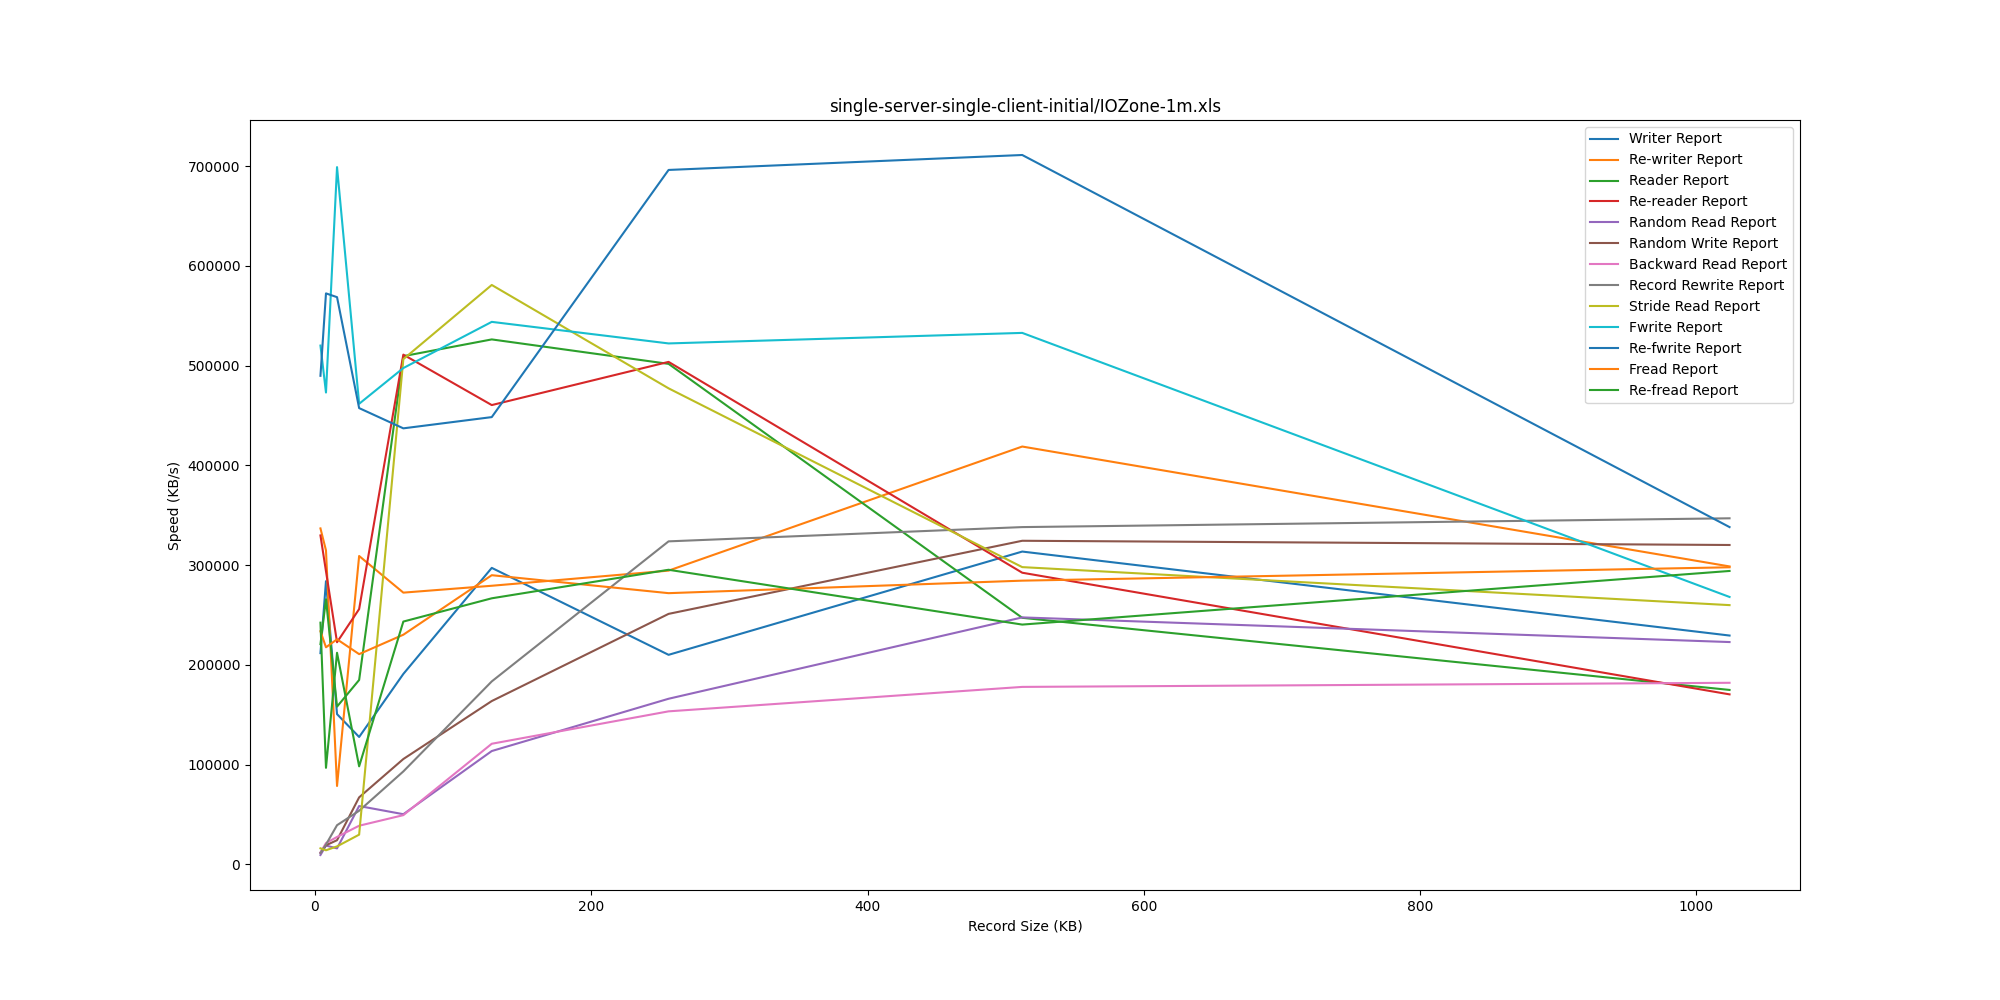
\includegraphics[width=\textwidth]{\baseimagedir/result/excel-to-chart/single-server-single-client-initial-IOZone-1m.xls.png}
    \caption{IOZone benchmark results on a single BeeGFS client node with a single node BeeGFS cluster mounted on it for 1MB file}
    \label{fig:signle-server-single-client-initial-1m}
\end{figure}

\begin{figure}
    \centering
    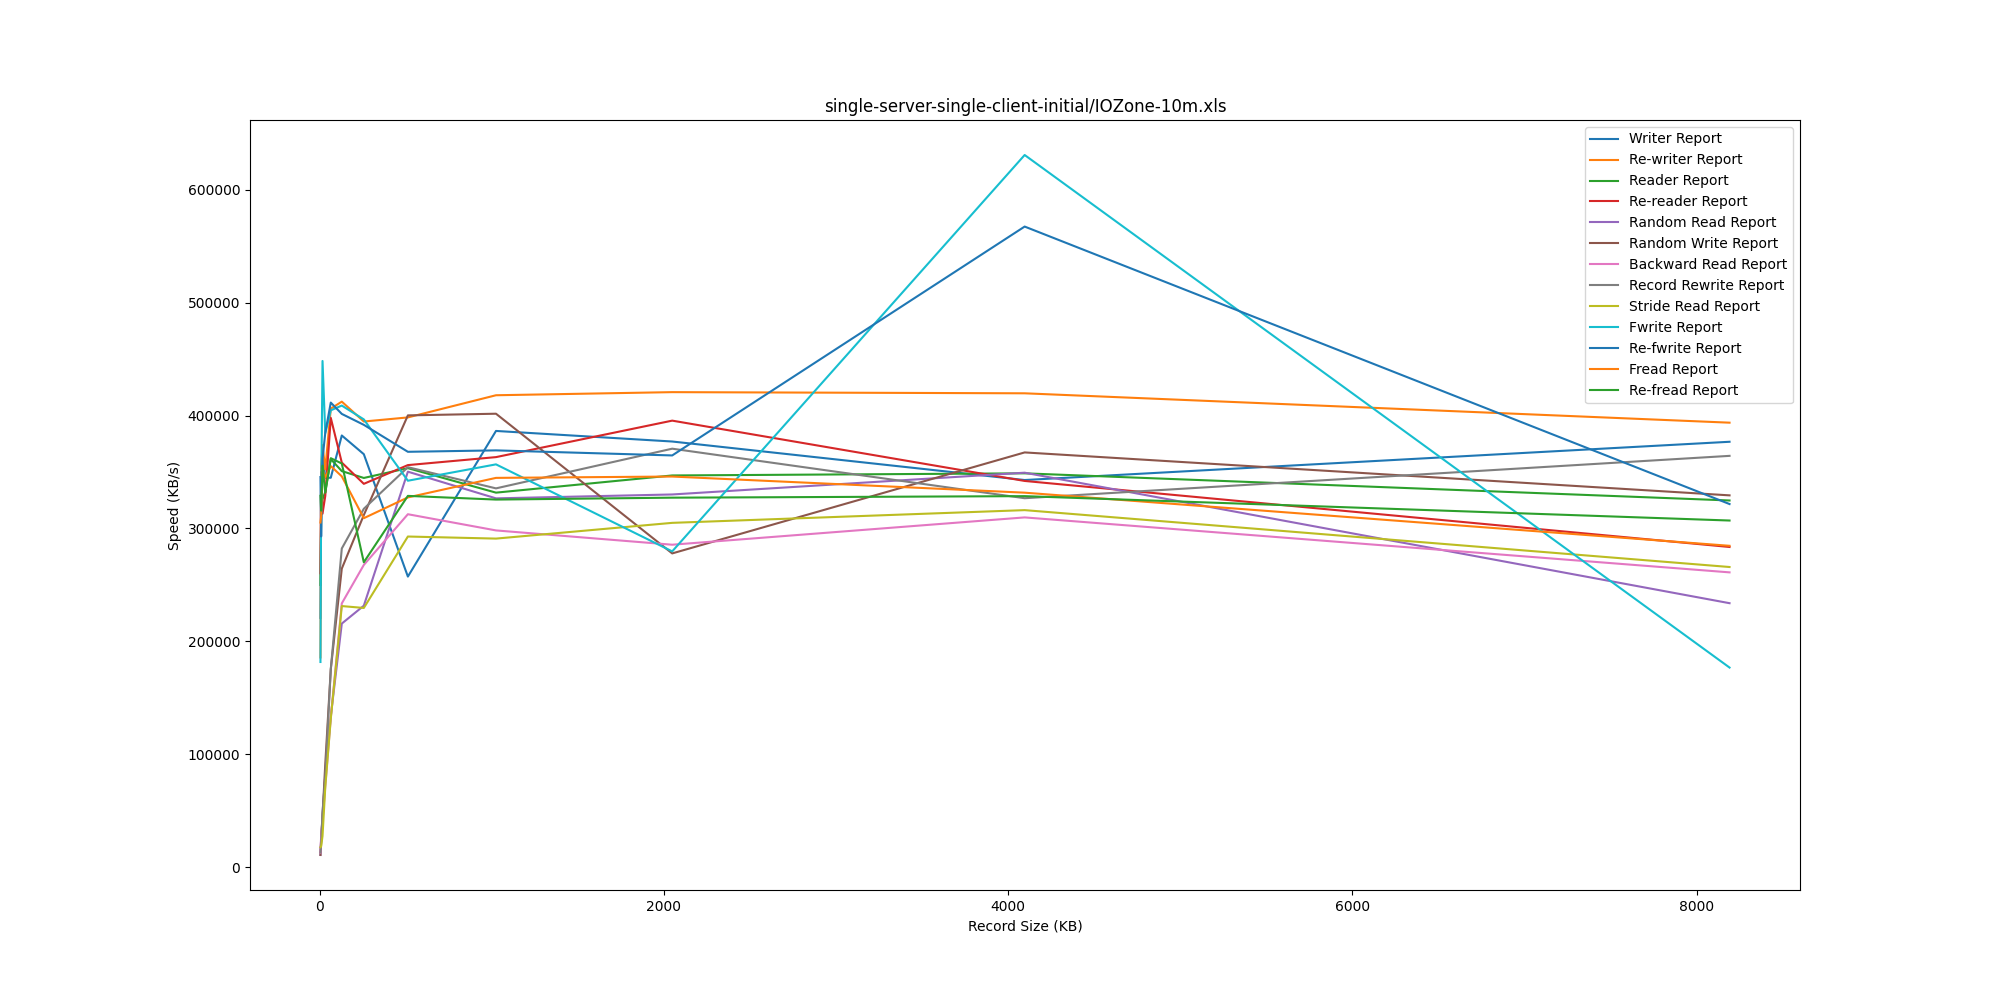
\includegraphics[width=\textwidth]{\baseimagedir/result/excel-to-chart/single-server-single-client-initial-IOZone-10m.xls.png}
    \caption{IOZone benchmark results on a single BeeGFS client node with a single node BeeGFS cluster mounted on it for 10MB file}
    \label{fig:signle-server-single-client-initial-10m}
\end{figure}

\begin{figure}
    \centering
    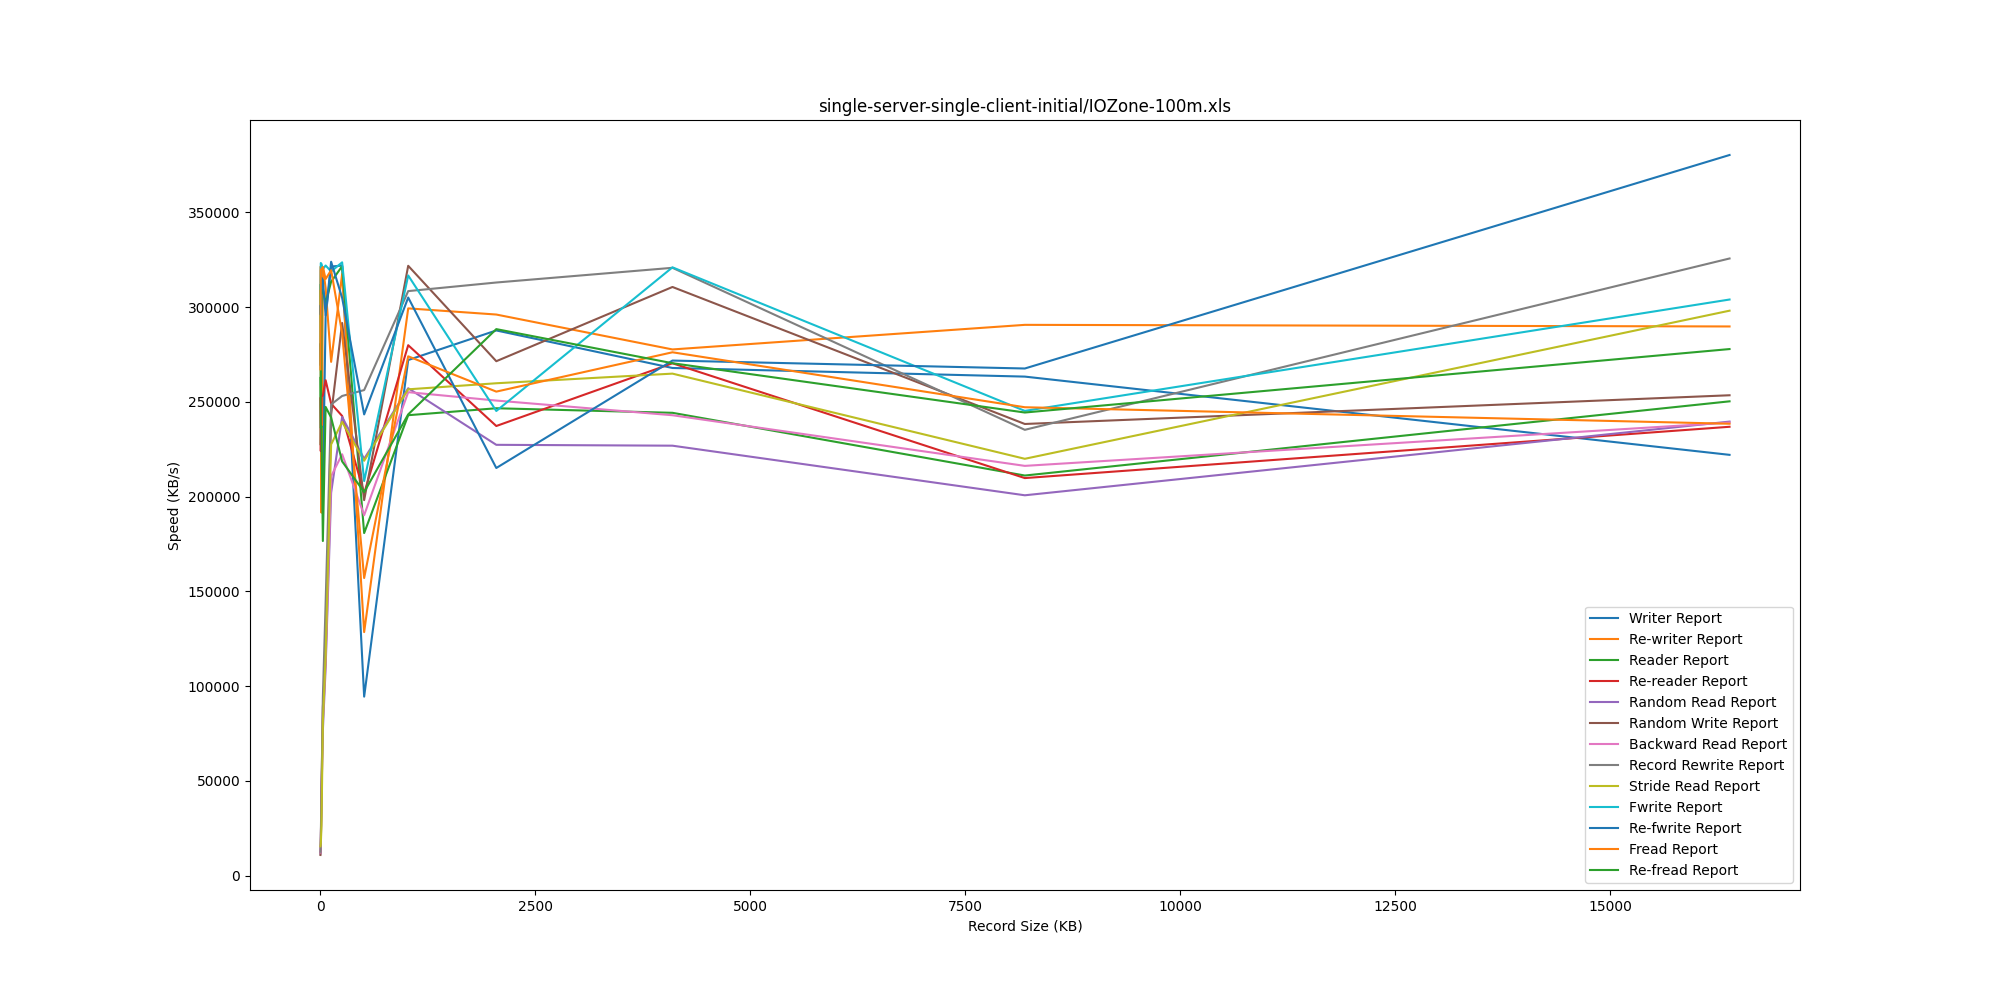
\includegraphics[width=\textwidth]{\baseimagedir/result/excel-to-chart/single-server-single-client-initial-IOZone-100m.xls.png}
    \caption{IOZone benchmark results on a single BeeGFS client node with a single node BeeGFS cluster mounted on it for 100MB file}
    \label{fig:signle-server-single-client-initial-100m}
\end{figure}

\begin{figure}
    \centering
    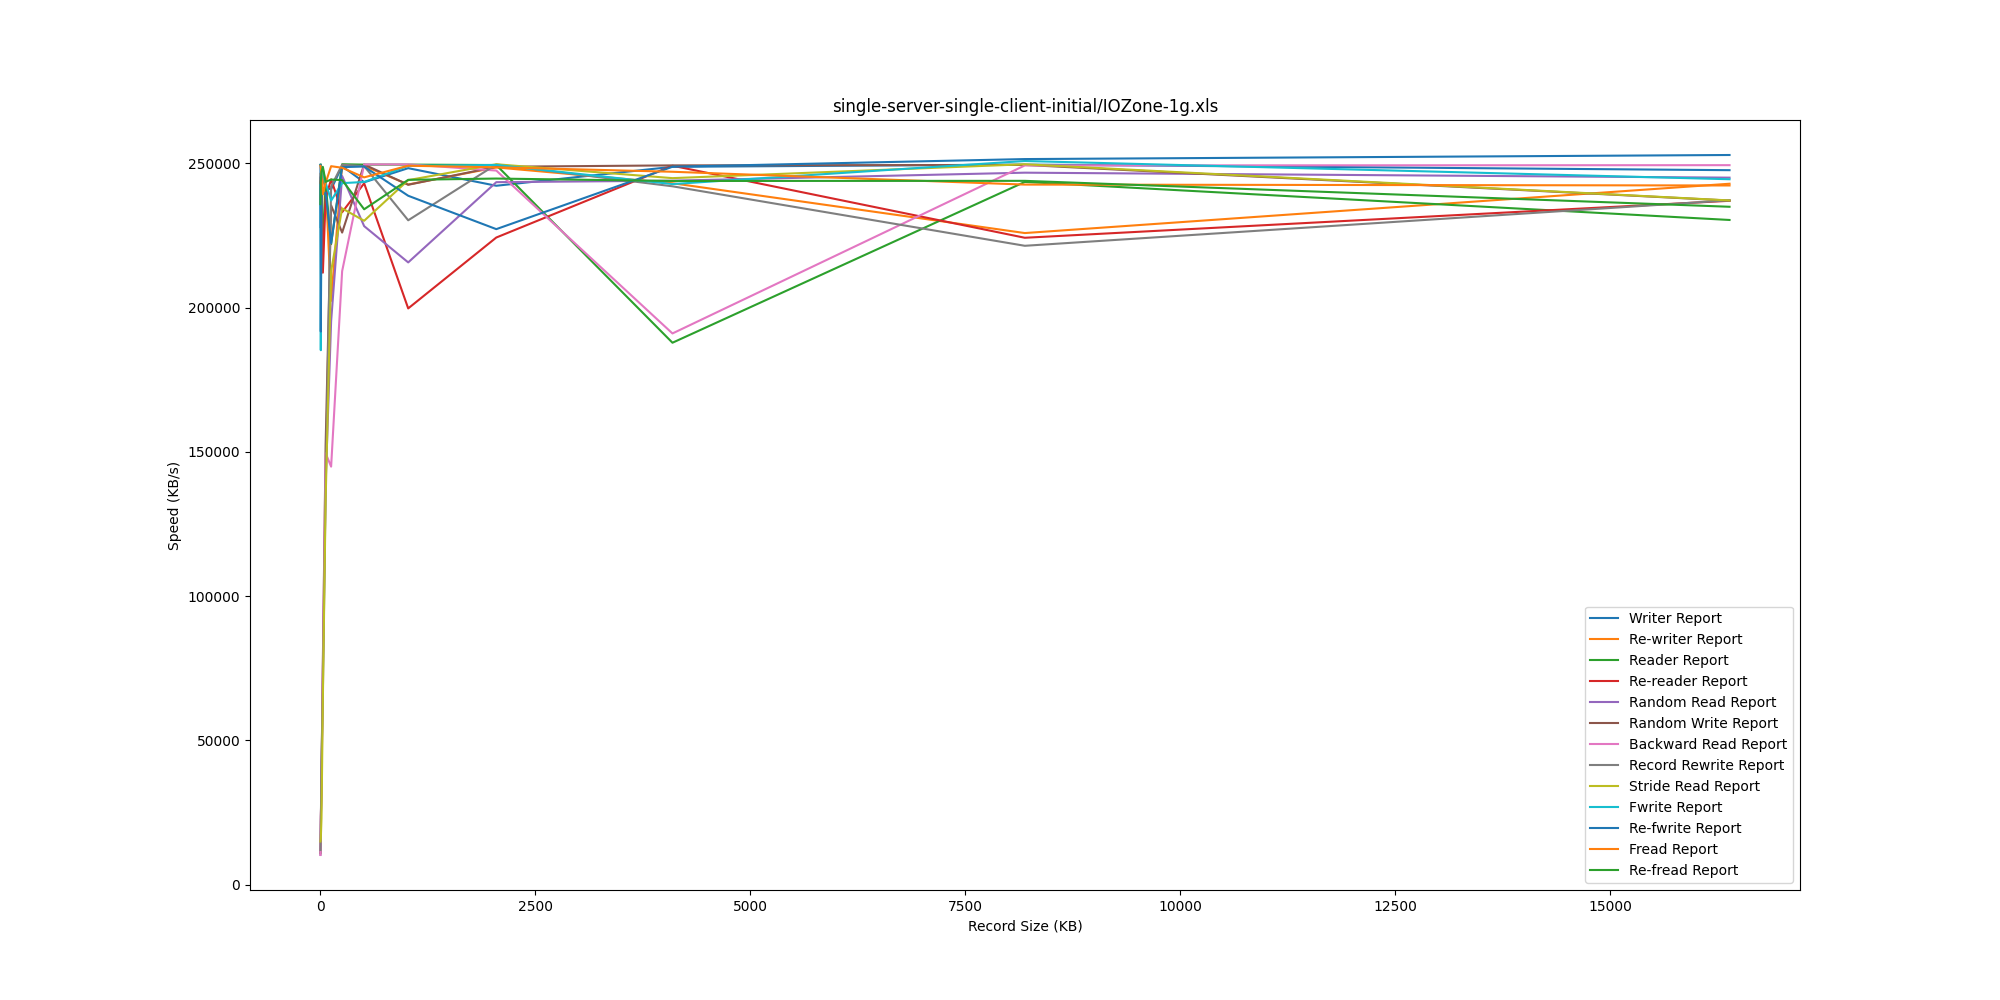
\includegraphics[width=\textwidth]{\baseimagedir/result/excel-to-chart/single-server-single-client-initial-IOZone-1g.xls.png}
    \caption{IOZone benchmark results on a single BeeGFS client node with a single node BeeGFS cluster mounted on it for 1GB file}
    \label{fig:signle-server-single-client-initial-1g}
\end{figure}

\begin{figure}
    \centering
    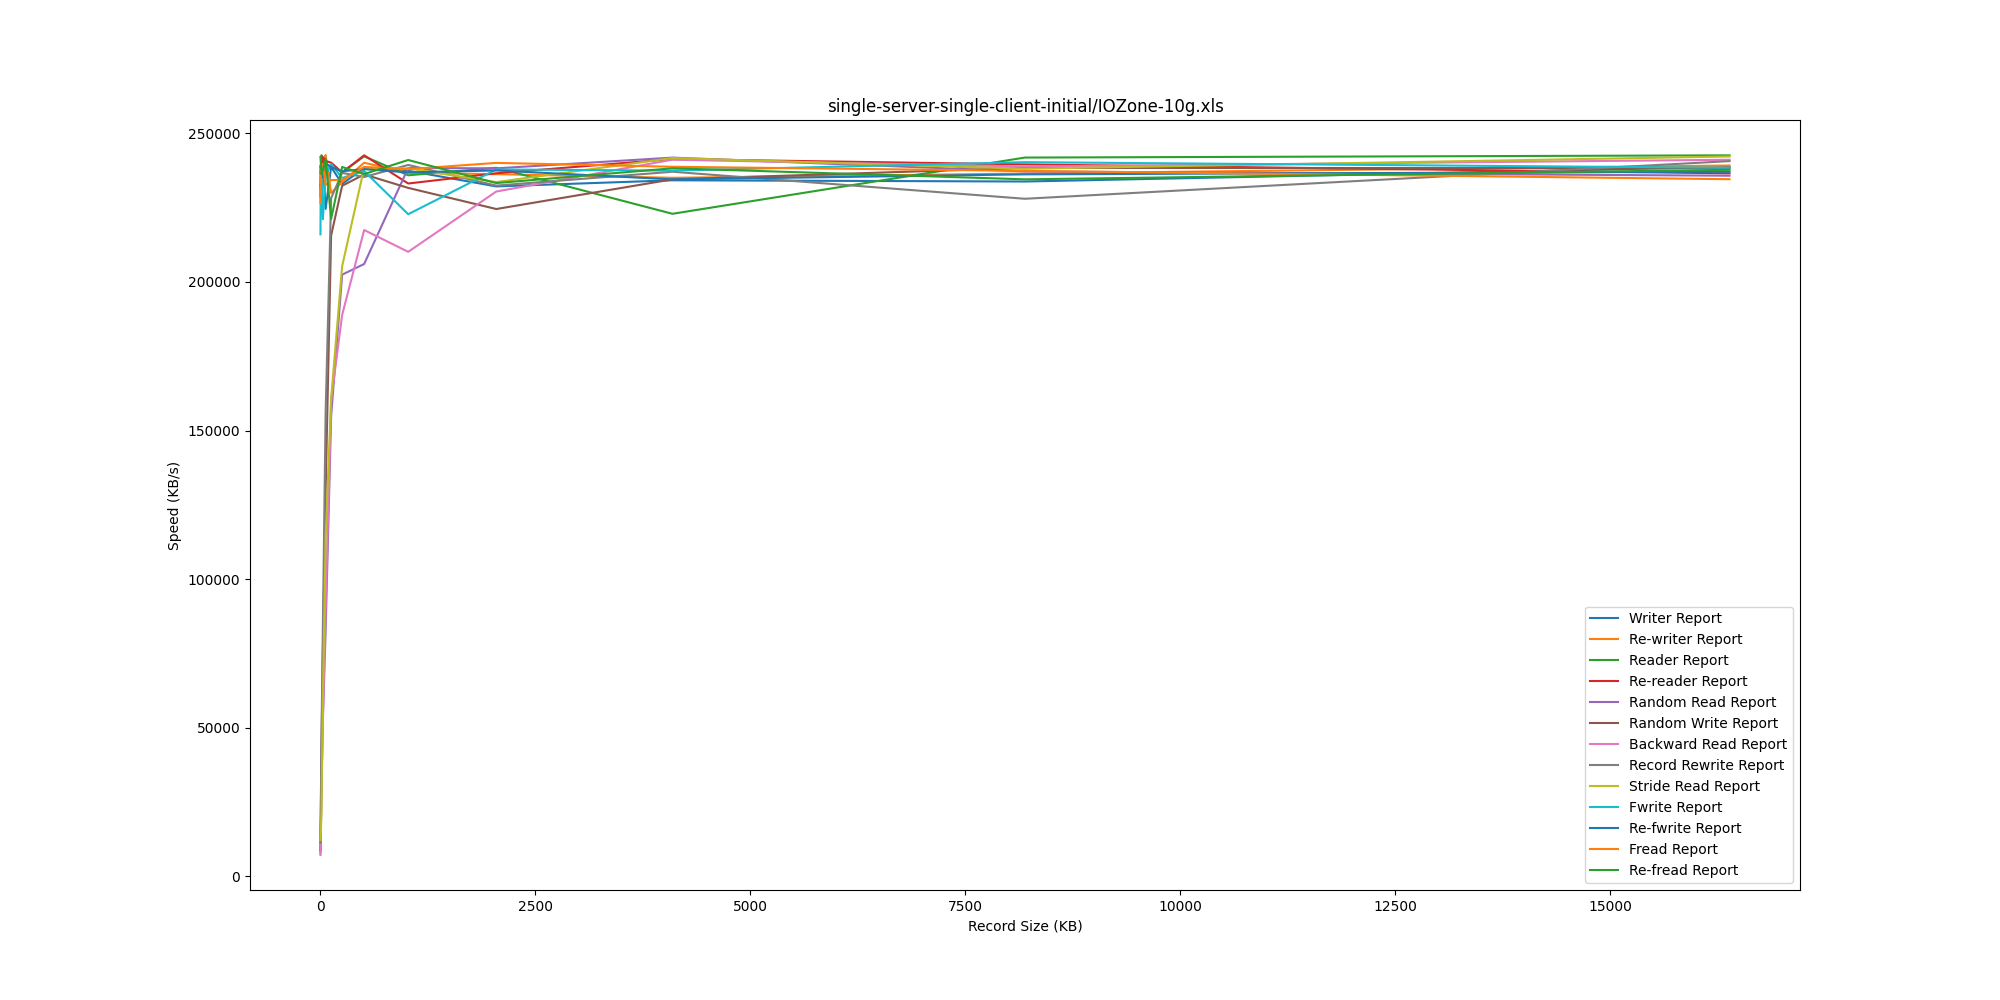
\includegraphics[width=\textwidth]{\baseimagedir/result/excel-to-chart/single-server-single-client-initial-IOZone-10g.xls.png}
    \caption{IOZone benchmark results on a single BeeGFS client node with a single node BeeGFS cluster mounted on it for 10GB file}
    \label{fig:signle-server-single-client-initial-10g}
\end{figure}


\section{Optimization and Tuning}
\subsection{Storage Tuning}
There are two sets of tuning done on the storage servers, one regarding memory and one regarding the storage disk.

\noindent Regarding the servers memory we did the following tunings:

\begin{itemize}
\item To avoid long IO stalls (latency) for write cache flushing we limited the kernel dirty write cache size
\item We also gave higher priority to inode caching to avoid disk seeks for inode loading
\item By Raising the amount of reserved kernel memory we achieved faster and more reliable memory allocation (Required for buffering of file system)
\item We also Enabled transparent hugepage for storage servers
\end{itemize}

\noindent Regarding the servers disks, we did the following tunings:

\begin{itemize}
    \item We first started by using Deadline Scheduler.
    \item We also increased request size of io queue for storage disks.
    \item Given our experiments, we had lots of sequential reads workloads, so we also had to tune disks for sequential reads.
    \item By increasing Max chunk size of each io request, we were able to reduce total amount of IO operations
\end{itemize}

The script used for doing such a tunings can be found in \texttt{tuning/storage-tuning.sh \footnote{\url{https://github.com/Parsa2820/BeeGFS-Benchmark/blob/master/tuning/storage-tuning.sh}}} file.

The result of the tuning for 1MB, 10MB, 100MB, 1GB, 10GB files can be seen in Figures \ref{fig:after-tune-1m}, \ref{fig:after-tune-10m}, \ref{fig:after-tune-100m}, \ref{fig:after-tune-1g}, \ref{fig:after-tune-10g} respectively. 

As we can see in the results, the performance of BeeGFS has improved significantly after the storage tuning. Especially for larger files.

\begin{figure}
    \centering
    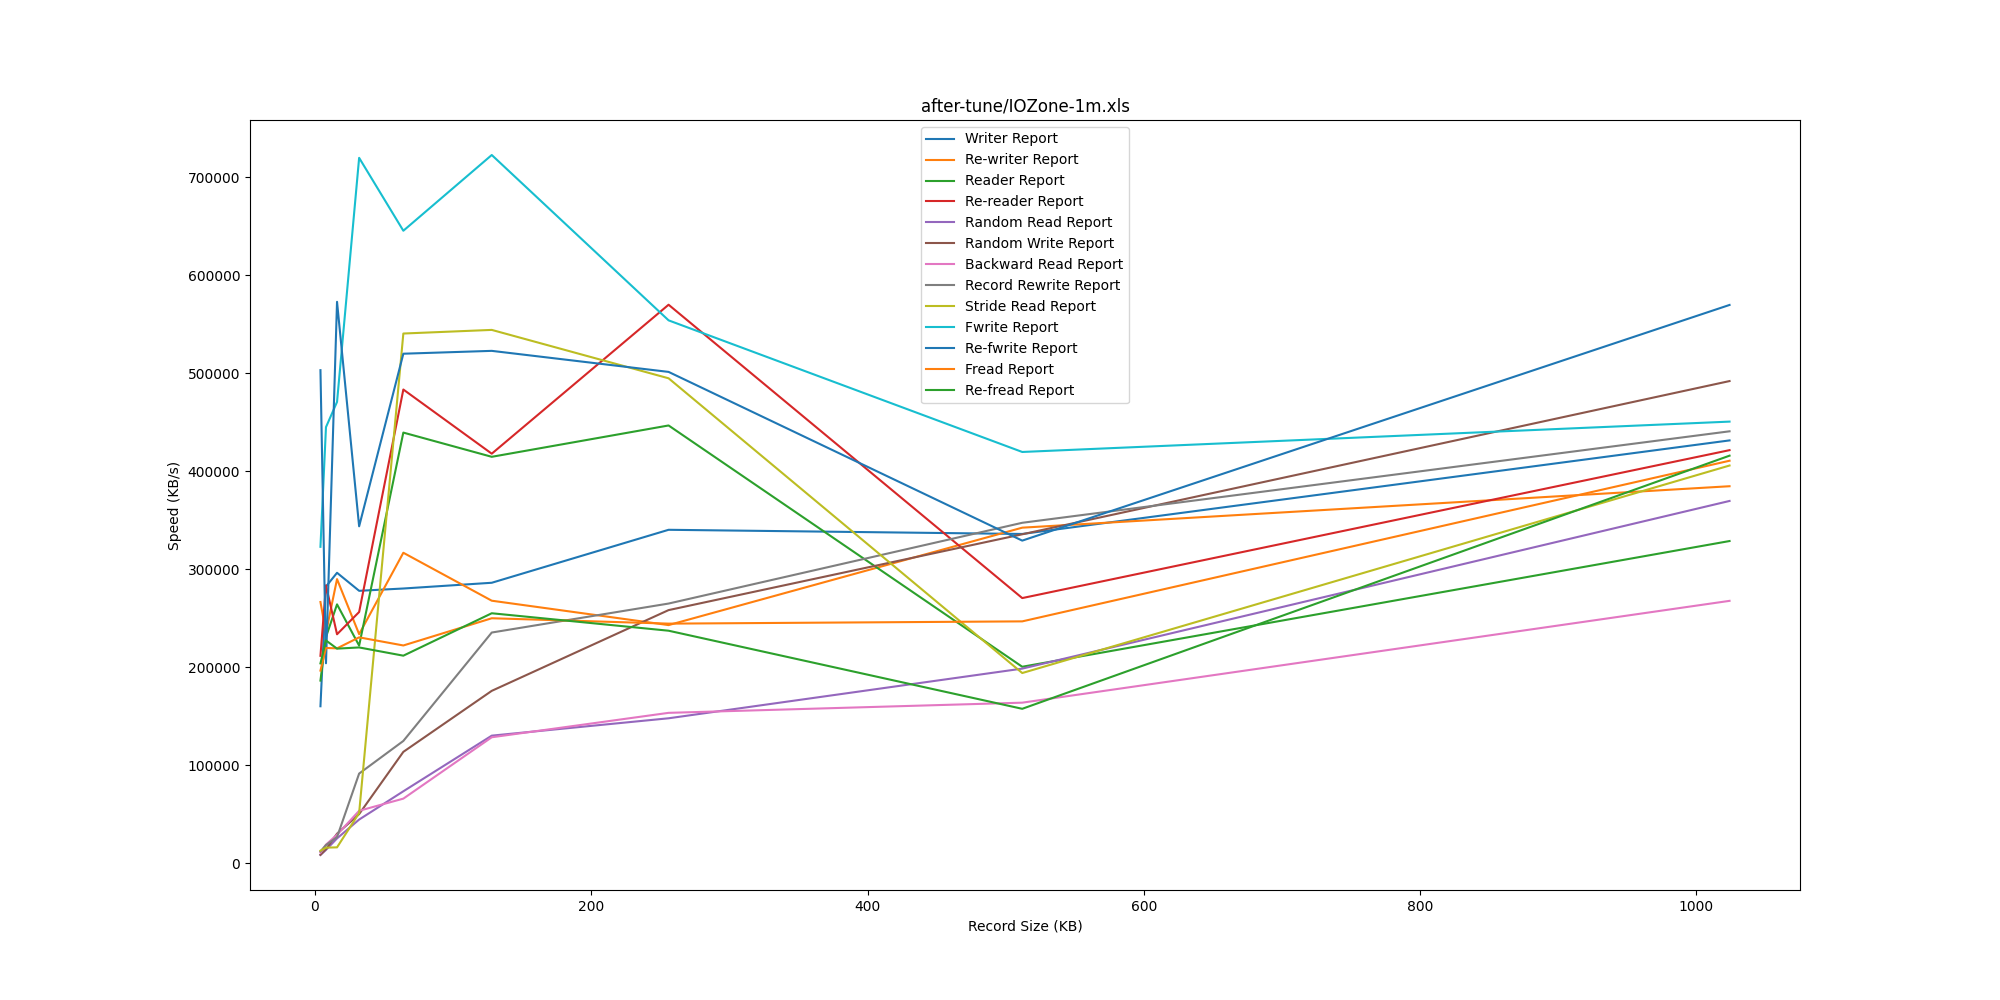
\includegraphics[width=\textwidth]{\baseimagedir/result/excel-to-chart/after-tune-IOZone-1m.xls.png}
    \caption{IOZone benchmark results for 1MB file after storage tuning}
    \label{fig:after-tune-1m}
\end{figure}

\begin{figure}
    \centering
    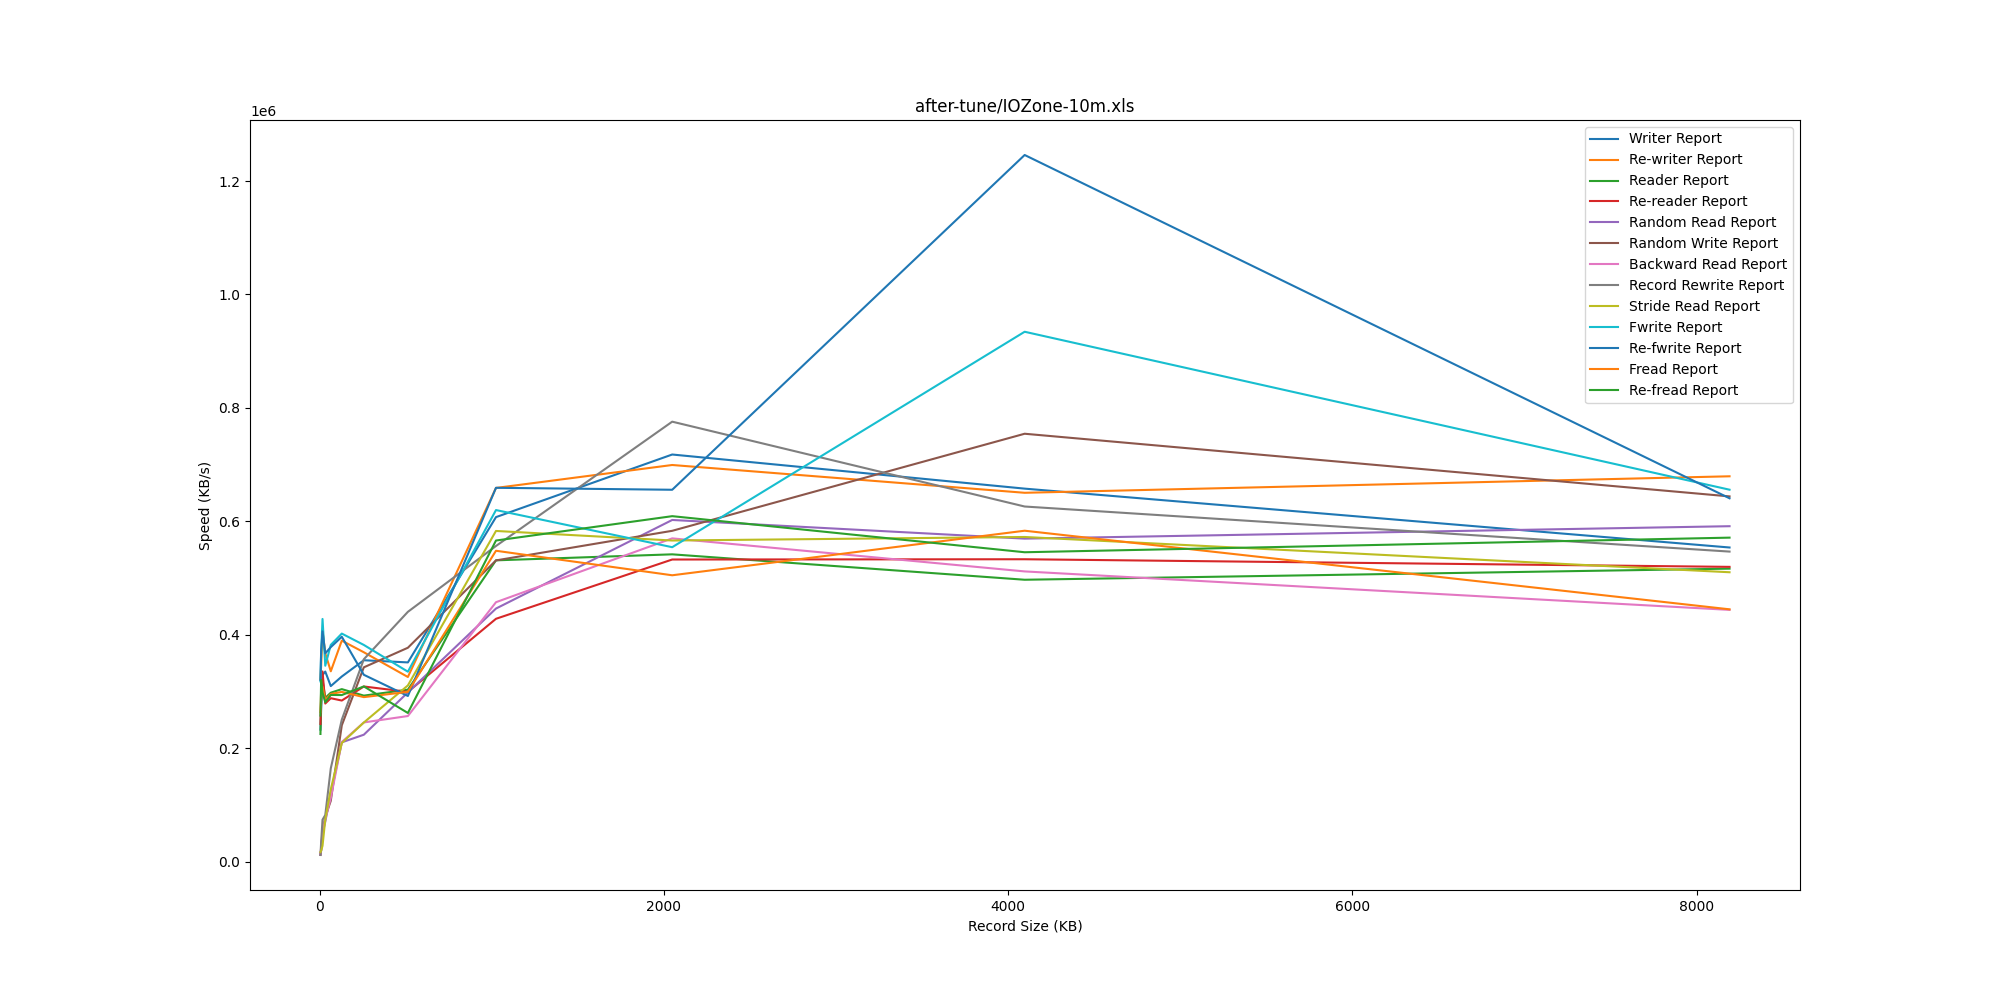
\includegraphics[width=\textwidth]{\baseimagedir/result/excel-to-chart/after-tune-IOZone-10m.xls.png}
    \caption{IOZone benchmark results for 10MB file after storage tuning}
    \label{fig:after-tune-10m}
\end{figure}

\begin{figure}
    \centering
    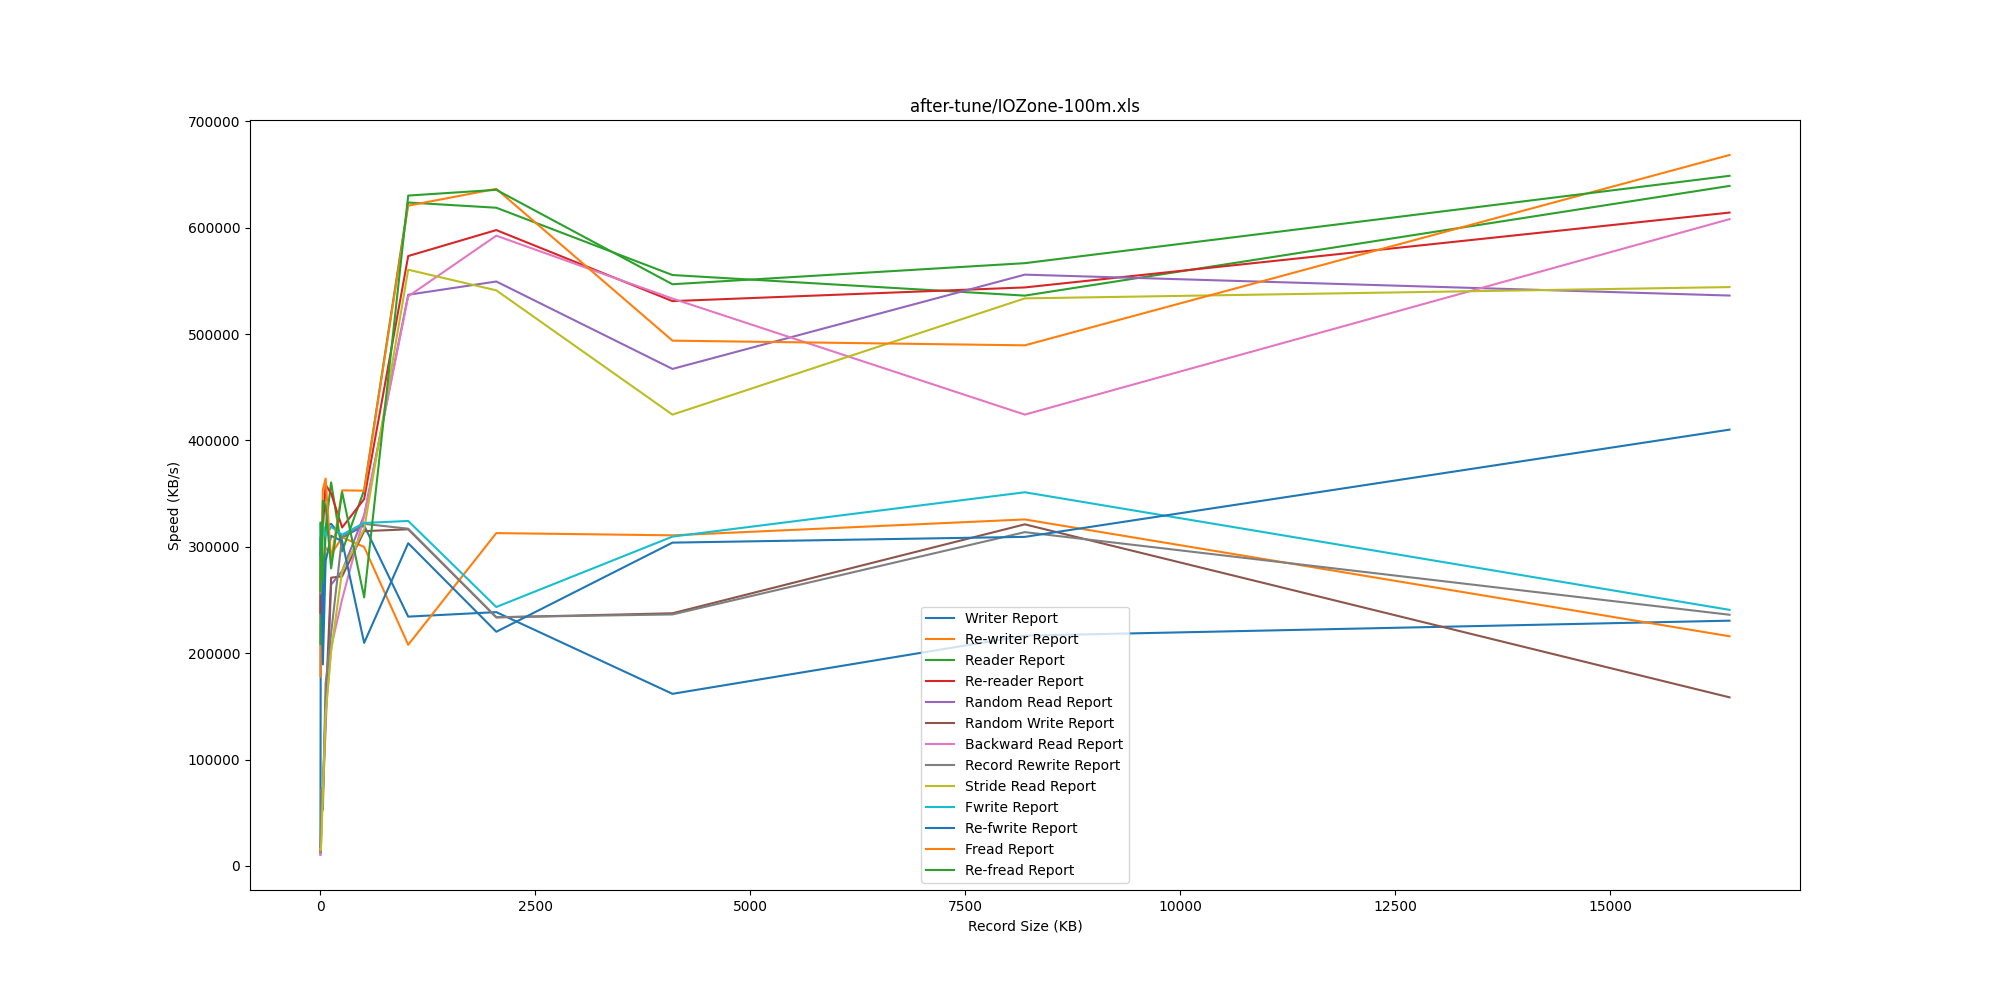
\includegraphics[width=\textwidth]{\baseimagedir/result/excel-to-chart/after-tune-IOZone-100m.xls.png}
    \caption{IOZone benchmark results for 100MB file after storage tuning}
    \label{fig:after-tune-100m}
\end{figure}

\begin{figure}
    \centering
    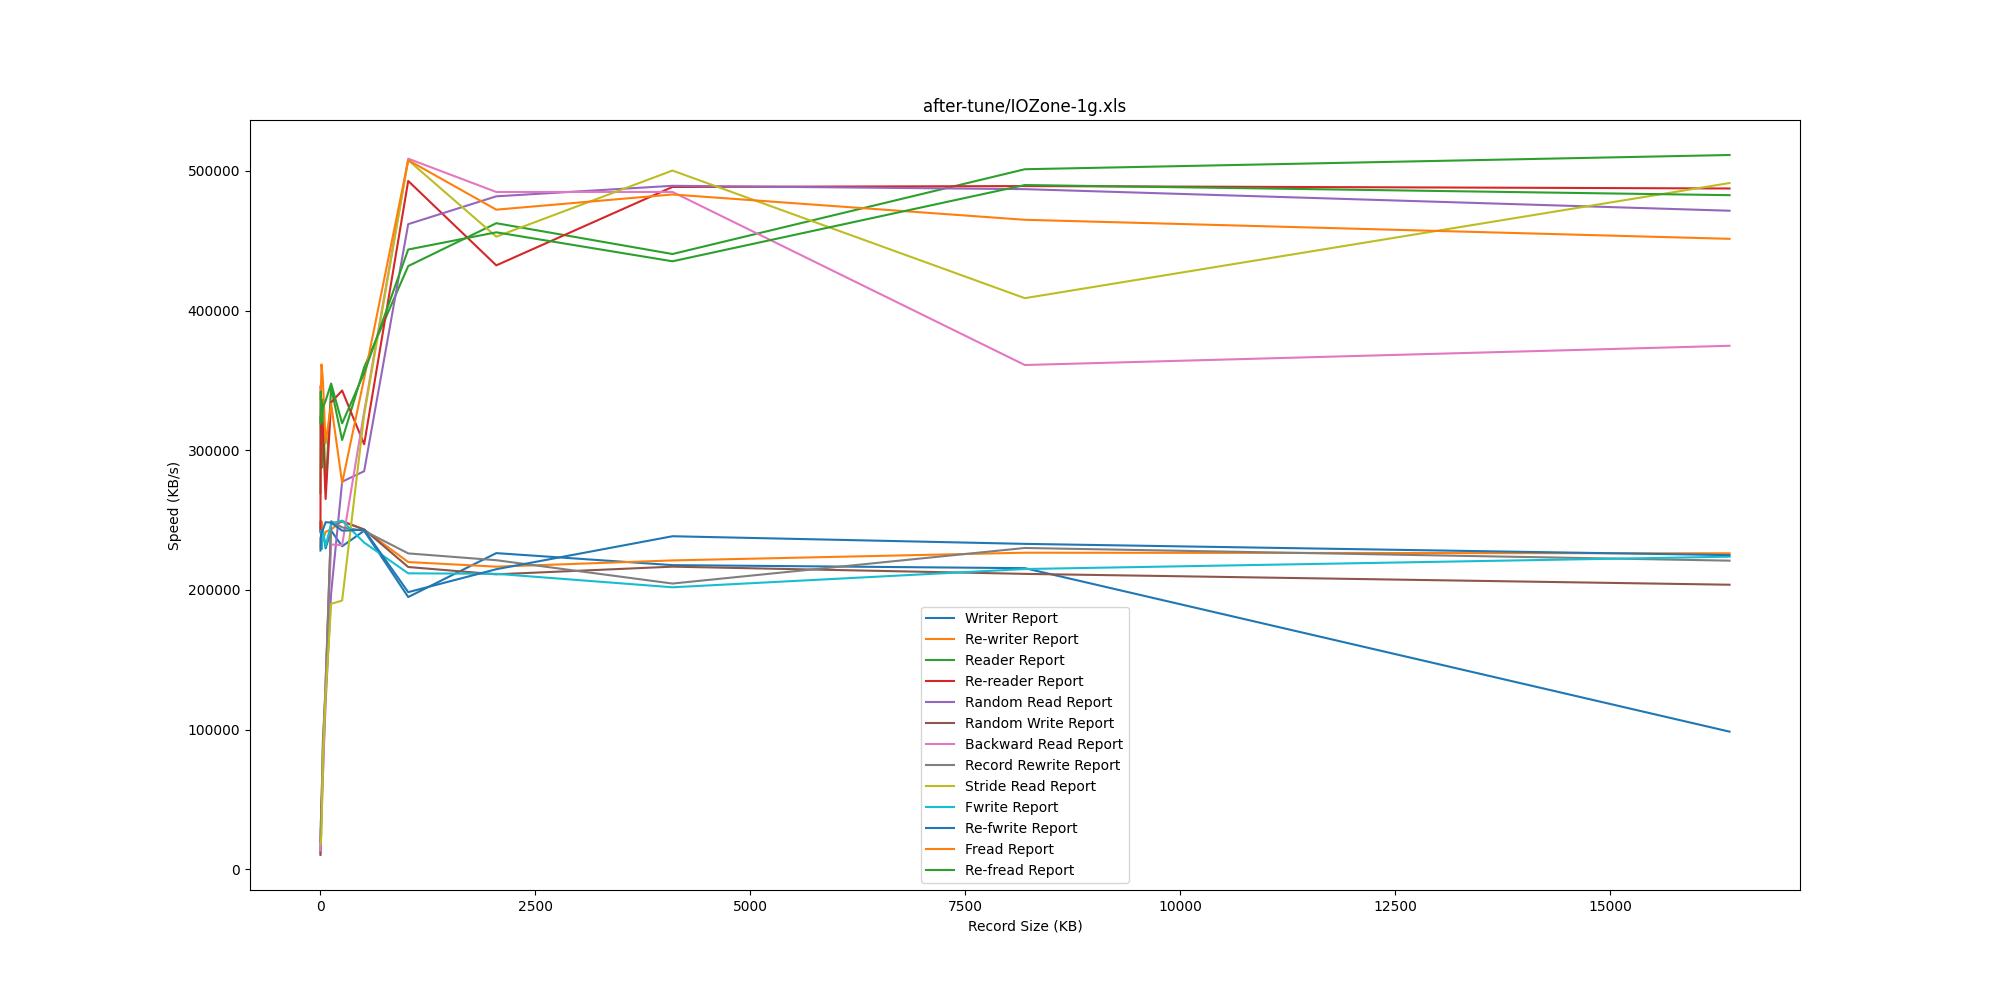
\includegraphics[width=\textwidth]{\baseimagedir/result/excel-to-chart/after-tune-IOZone-1g.xls.png}
    \caption{IOZone benchmark results for 1GB file after storage tuning}
    \label{fig:after-tune-1g}
\end{figure}

\begin{figure}
    \centering
    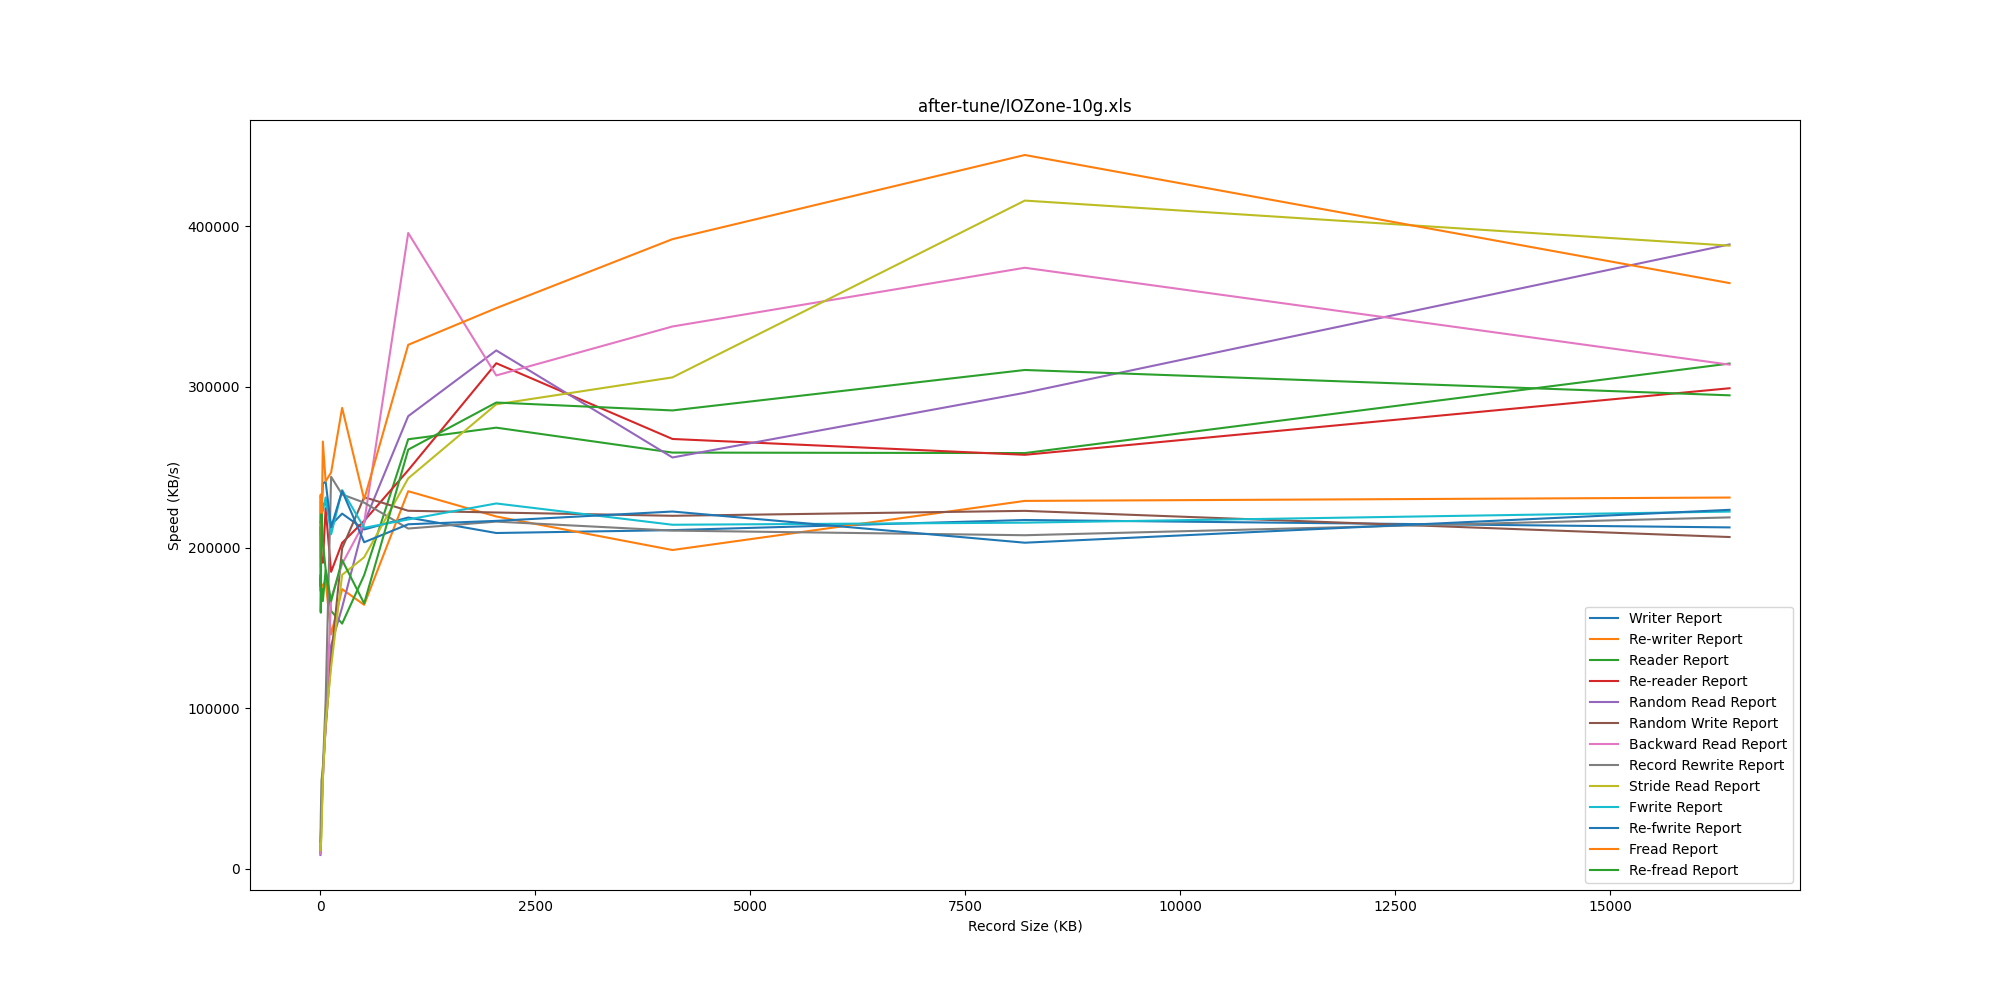
\includegraphics[width=\textwidth]{\baseimagedir/result/excel-to-chart/after-tune-IOZone-10g.xls.png}
    \caption{IOZone benchmark results for 10GB file after storage tuning}
    \label{fig:after-tune-10g}
\end{figure}

\subsection{Data Stripping}
In order to Improve the overall performance of the system, BeeGFS recommends the usage of stripping in file system. We conducted an experiment to measure the effectiveness of stripping on IO performance. BeeGFS provides a per directory stripping configuration. We created 4 directories, named s1 to s4, each with stripping level of 1 to 4 receptively.

The results of the experiment in the s1 directory for 1MB, 10MB, 100MB files can be seen in Figures \ref{fig:s1-1m}, \ref{fig:s1-10m}, \ref{fig:s1-100m} respectively. The results of the experiment in the s2 directory for 1MB, 10MB, 100MB files can be seen in Figures \ref{fig:s2-1m}, \ref{fig:s2-10m}, \ref{fig:s2-100m} respectively. The results of the experiment in the s3 directory for 1MB, 10MB, 100MB files can be seen in Figures \ref{fig:s3-1m}, \ref{fig:s3-10m}, \ref{fig:s3-100m} respectively. The results of the experiment in the s4 directory for 1MB, 10MB, 100MB files can be seen in Figures \ref{fig:s4-1m}, \ref{fig:s4-10m}, \ref{fig:s4-100m} respectively.

As we can see in the results, even levels of stripping have absolutely better performance than odd levels of stripping. The size of the files has its effect on the performance, but the previous statement is true for all file sizes. 

\begin{figure}
    \centering
    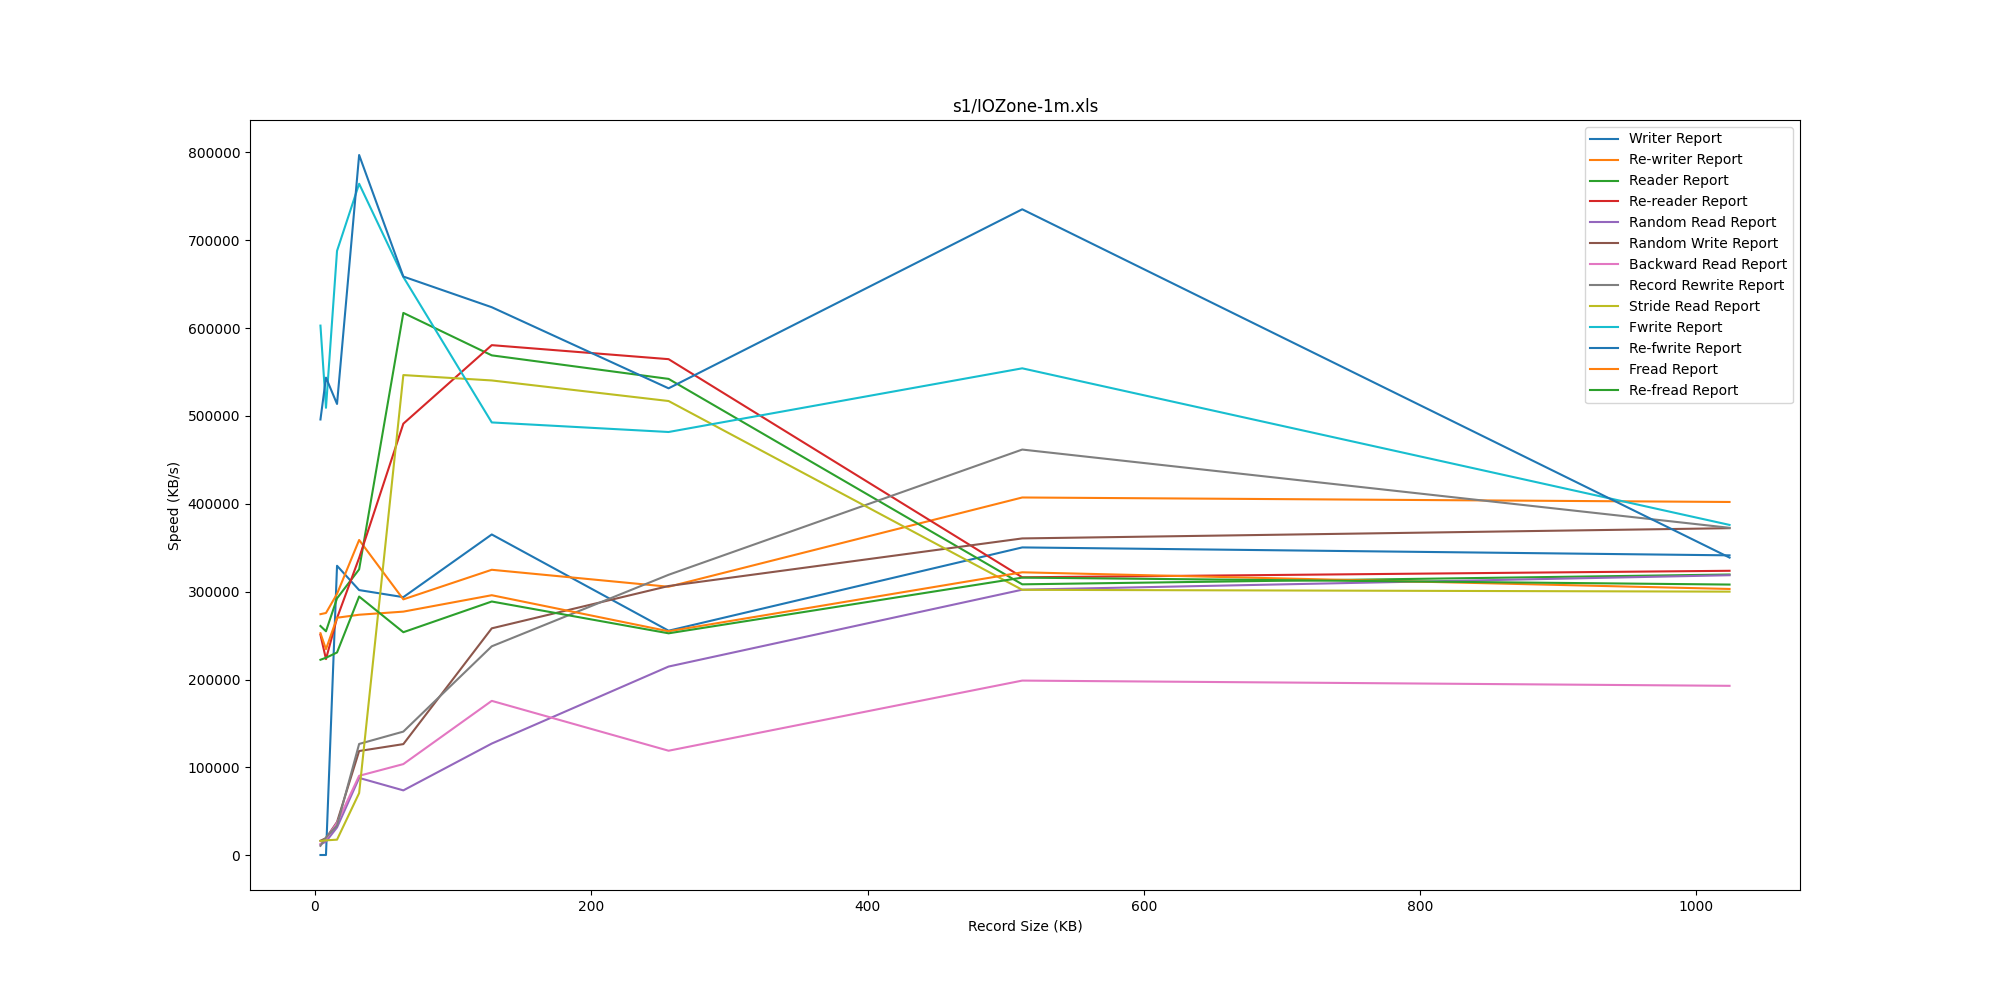
\includegraphics[width=\textwidth]{\baseimagedir/result/excel-to-chart/s1-IOZone-1m.xls.png}
    \caption{IOZone benchmark results for 1MB file in s1 directory}
    \label{fig:s1-1m}
\end{figure}

\begin{figure}
    \centering
    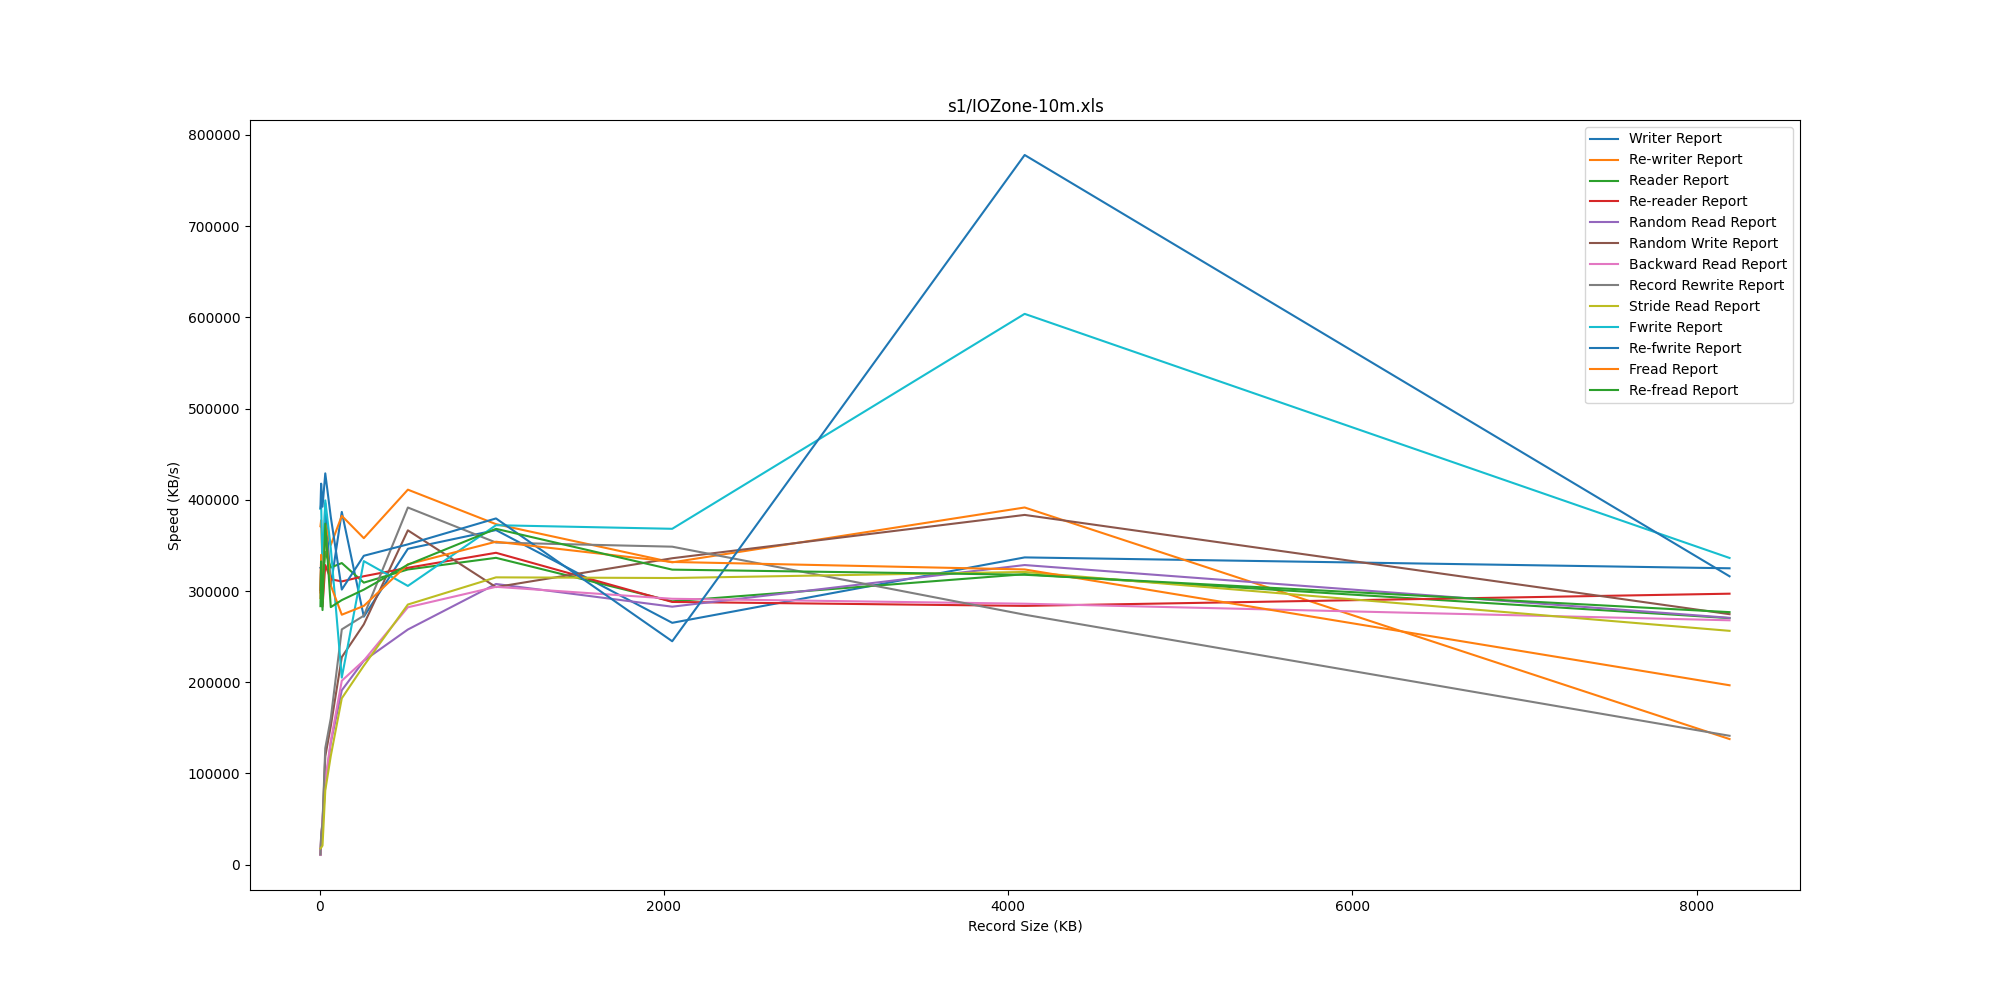
\includegraphics[width=\textwidth]{\baseimagedir/result/excel-to-chart/s1-IOZone-10m.xls.png}
    \caption{IOZone benchmark results for 10MB file in s1 directory}
    \label{fig:s1-10m}
\end{figure}

\begin{figure}
    \centering
    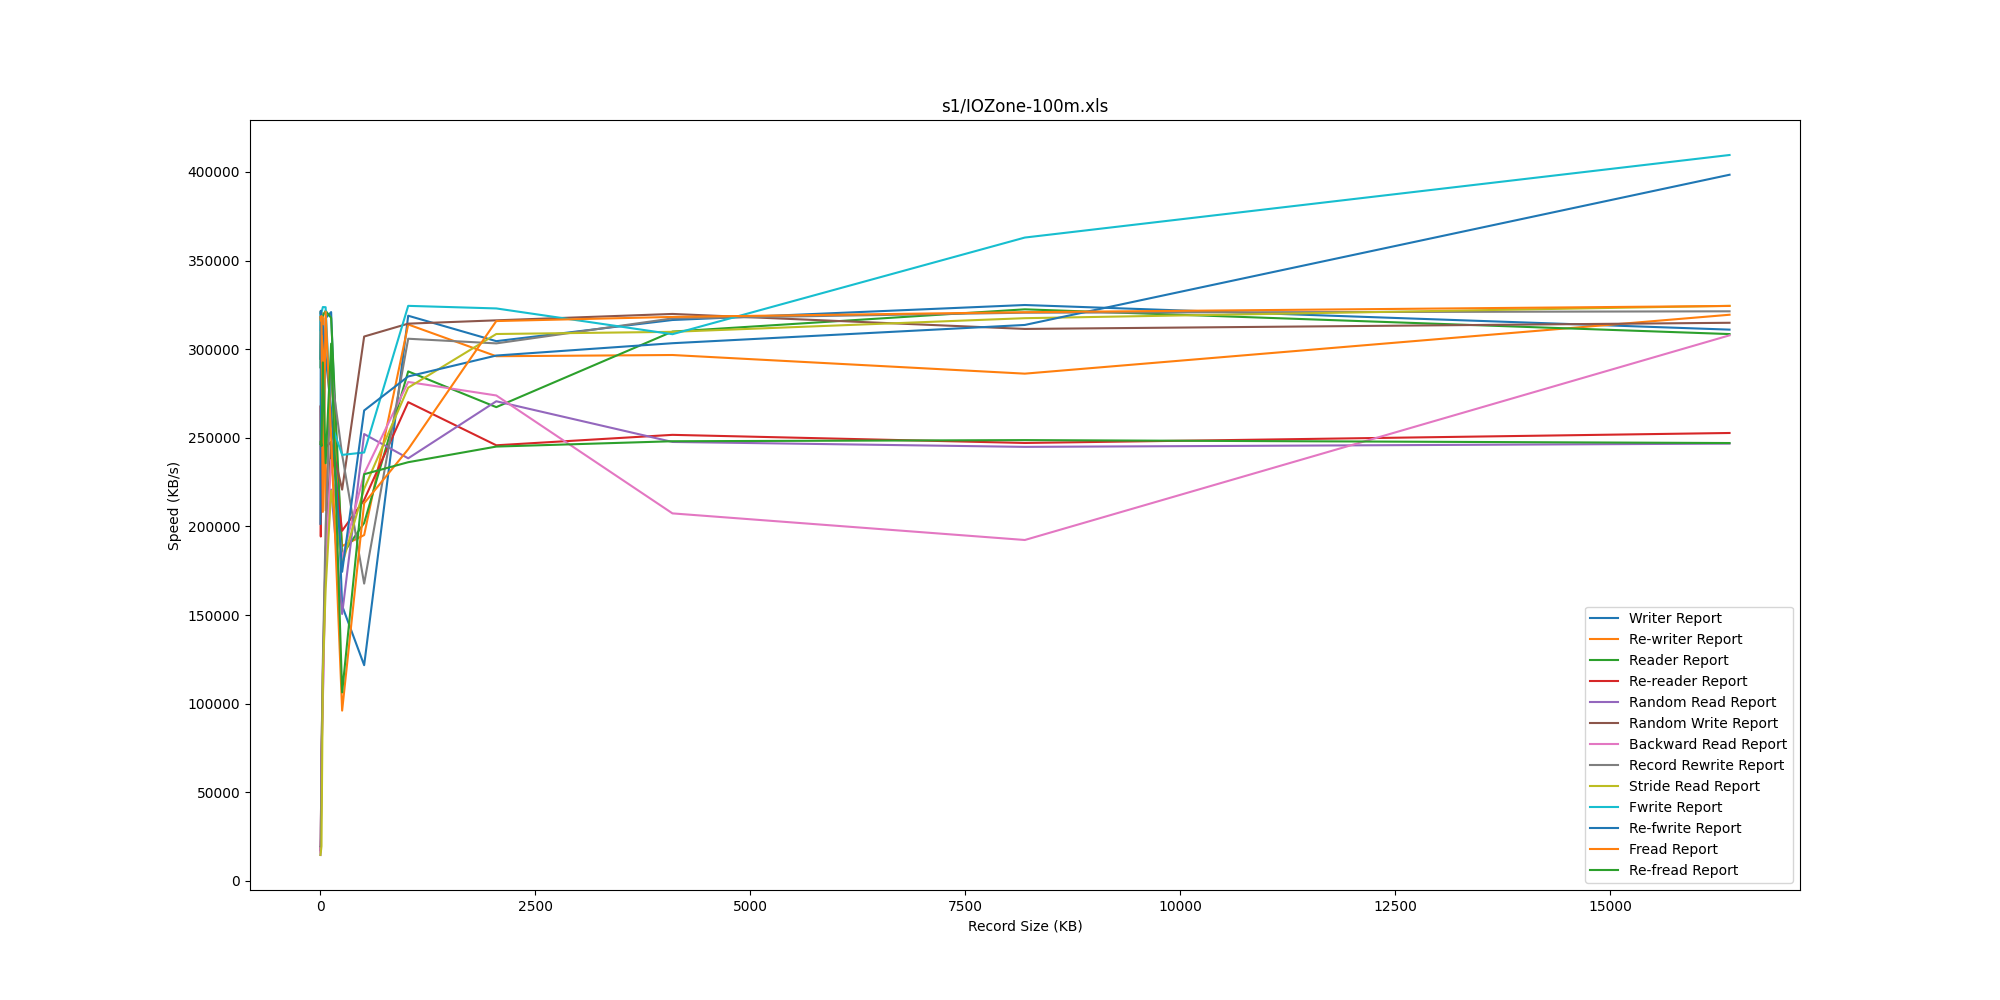
\includegraphics[width=\textwidth]{\baseimagedir/result/excel-to-chart/s1-IOZone-100m.xls.png}
    \caption{IOZone benchmark results for 100MB file in s1 directory}
    \label{fig:s1-100m}
\end{figure}

\begin{figure}
    \centering
    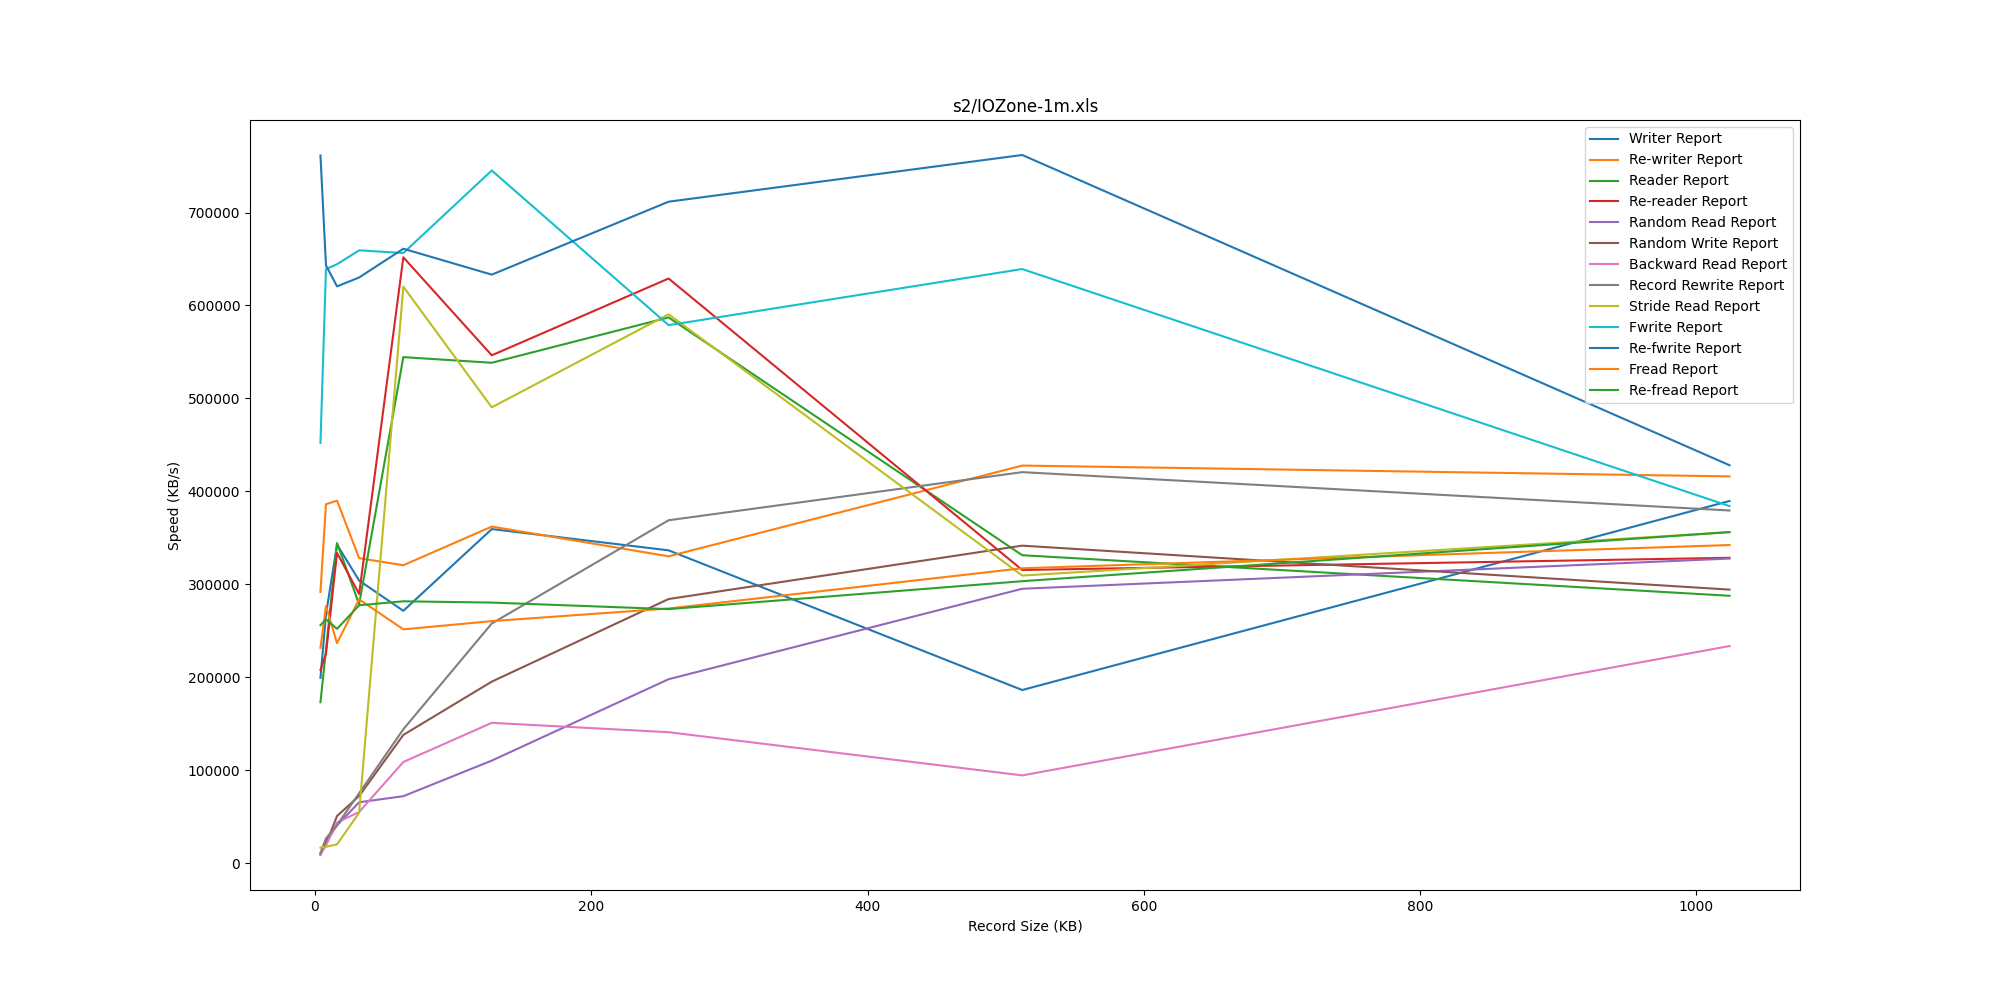
\includegraphics[width=\textwidth]{\baseimagedir/result/excel-to-chart/s2-IOZone-1m.xls.png}
    \caption{IOZone benchmark results for 1MB file in s2 directory}
    \label{fig:s2-1m}
\end{figure}

\begin{figure}
    \centering
    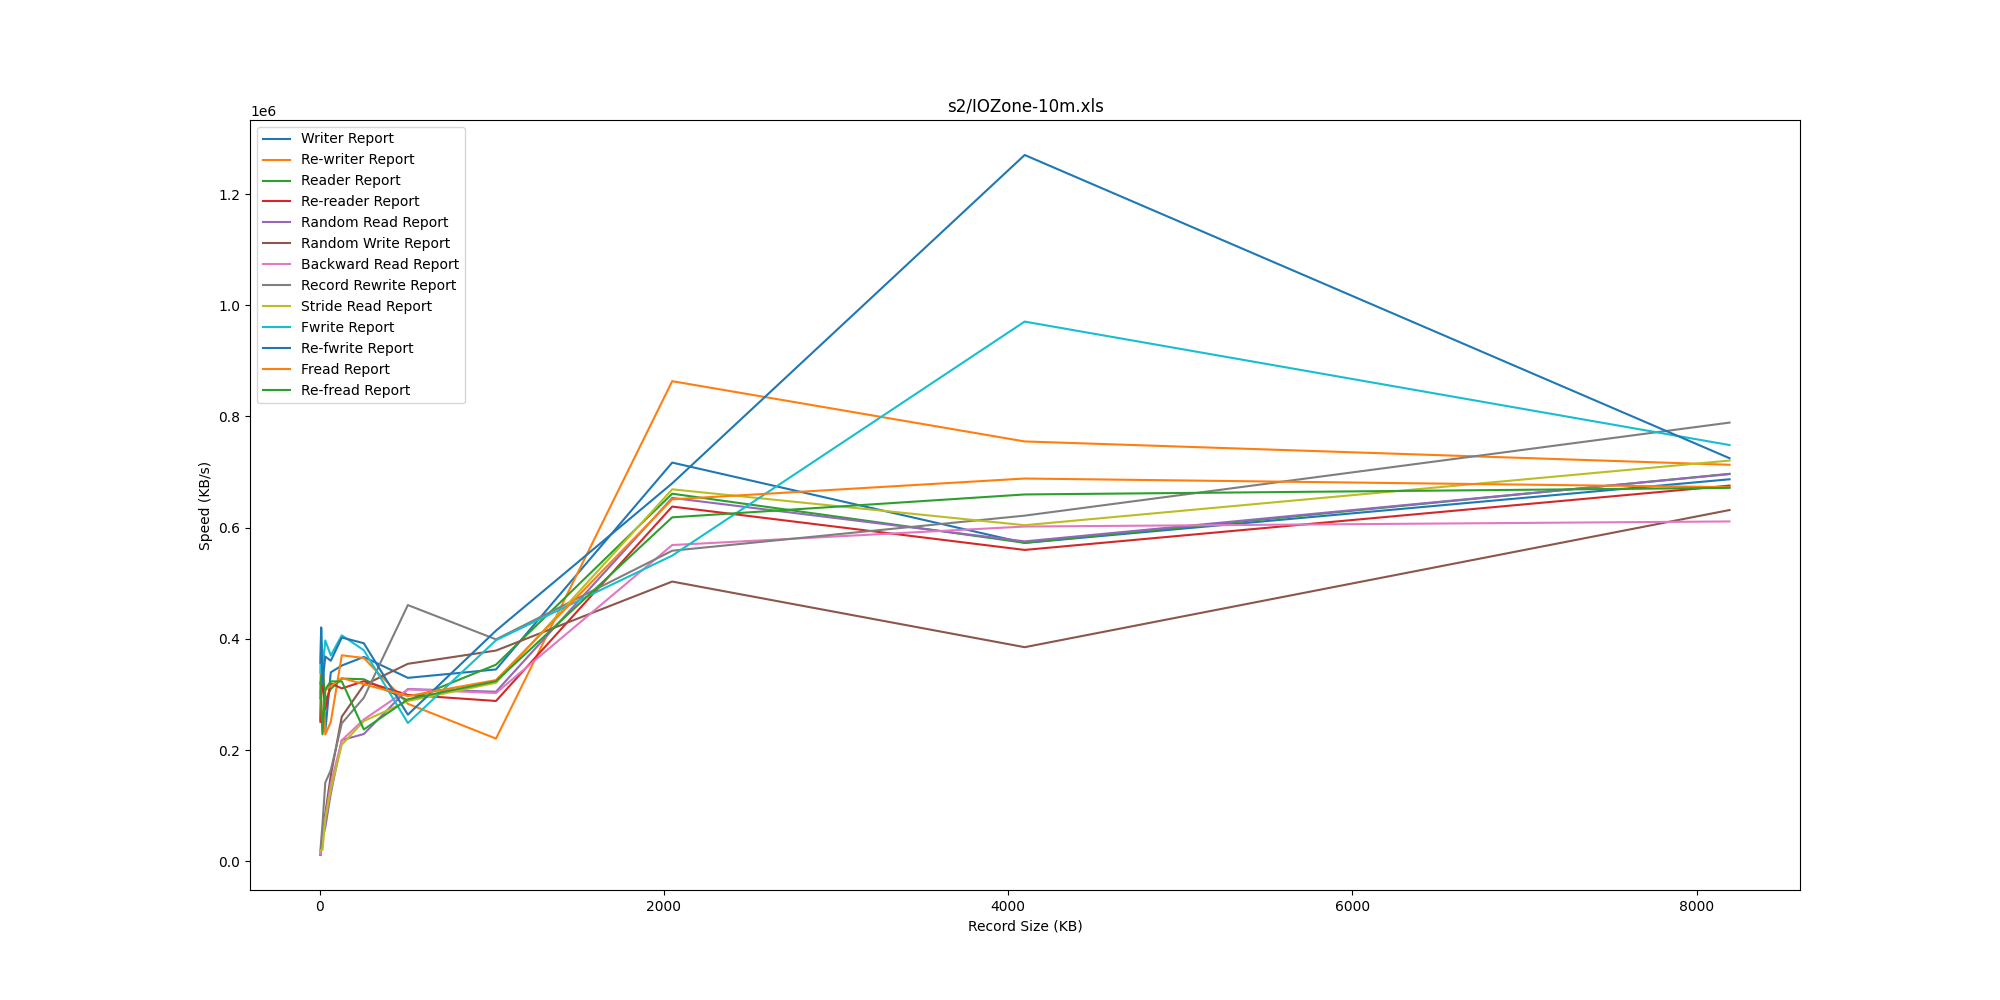
\includegraphics[width=\textwidth]{\baseimagedir/result/excel-to-chart/s2-IOZone-10m.xls.png}
    \caption{IOZone benchmark results for 10MB file in s2 directory}
    \label{fig:s2-10m}
\end{figure}

\begin{figure}
    \centering
    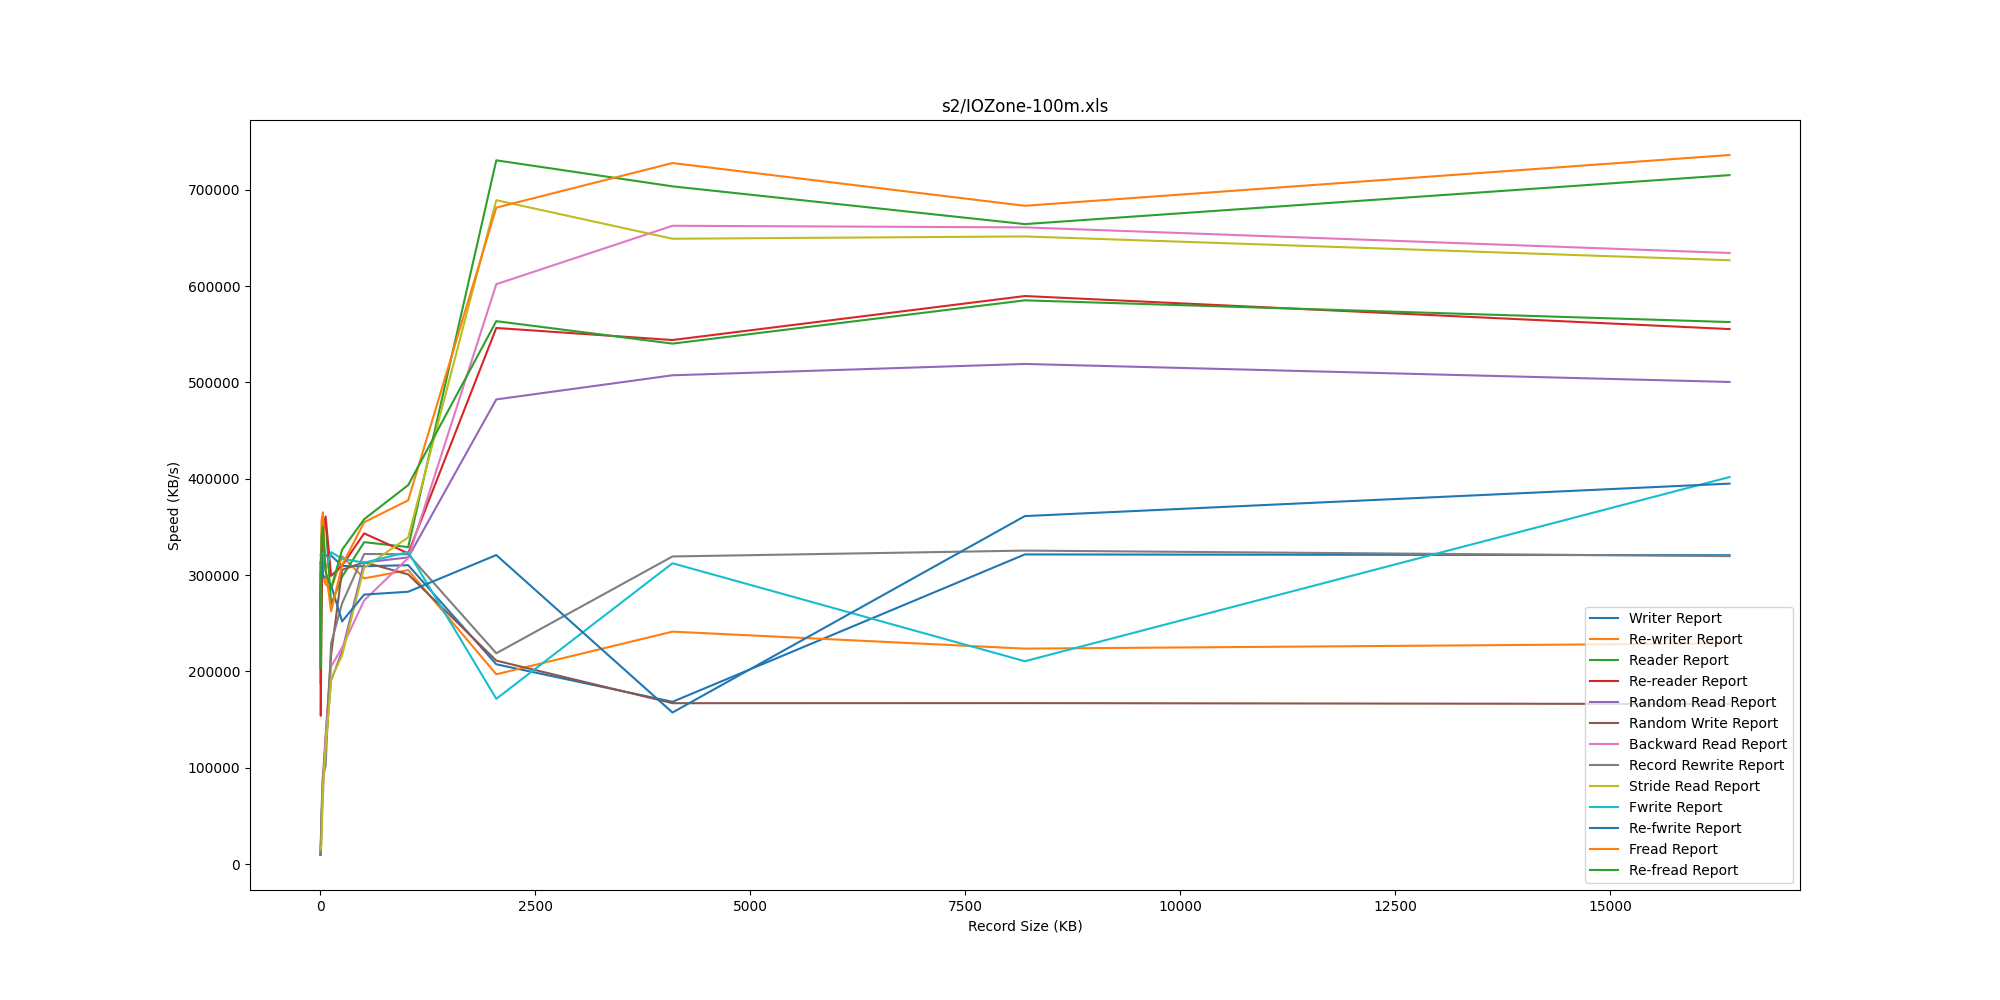
\includegraphics[width=\textwidth]{\baseimagedir/result/excel-to-chart/s2-IOZone-100m.xls.png}
    \caption{IOZone benchmark results for 100MB file in s2 directory}
    \label{fig:s2-100m}
\end{figure}

\begin{figure}
    \centering
    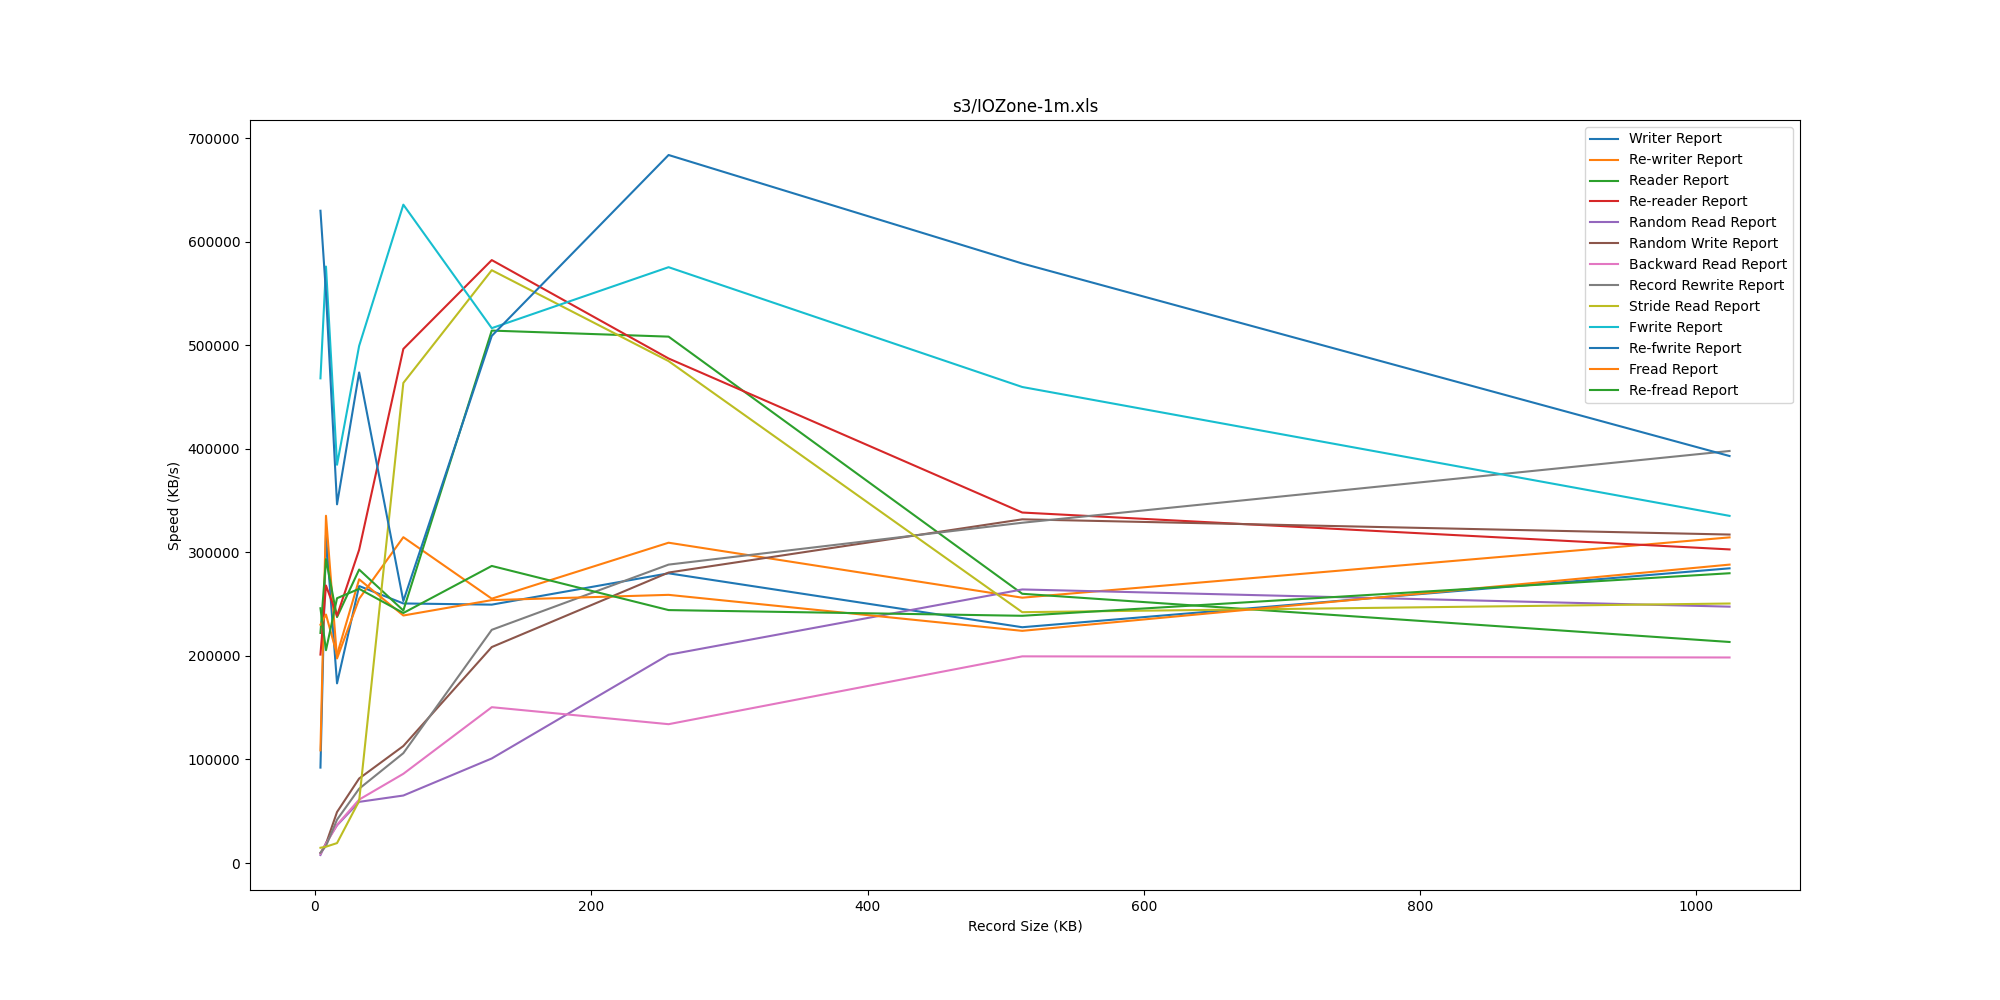
\includegraphics[width=\textwidth]{\baseimagedir/result/excel-to-chart/s3-IOZone-1m.xls.png}
    \caption{IOZone benchmark results for 1MB file in s3 directory}
    \label{fig:s3-1m}
\end{figure}

\begin{figure}
    \centering
    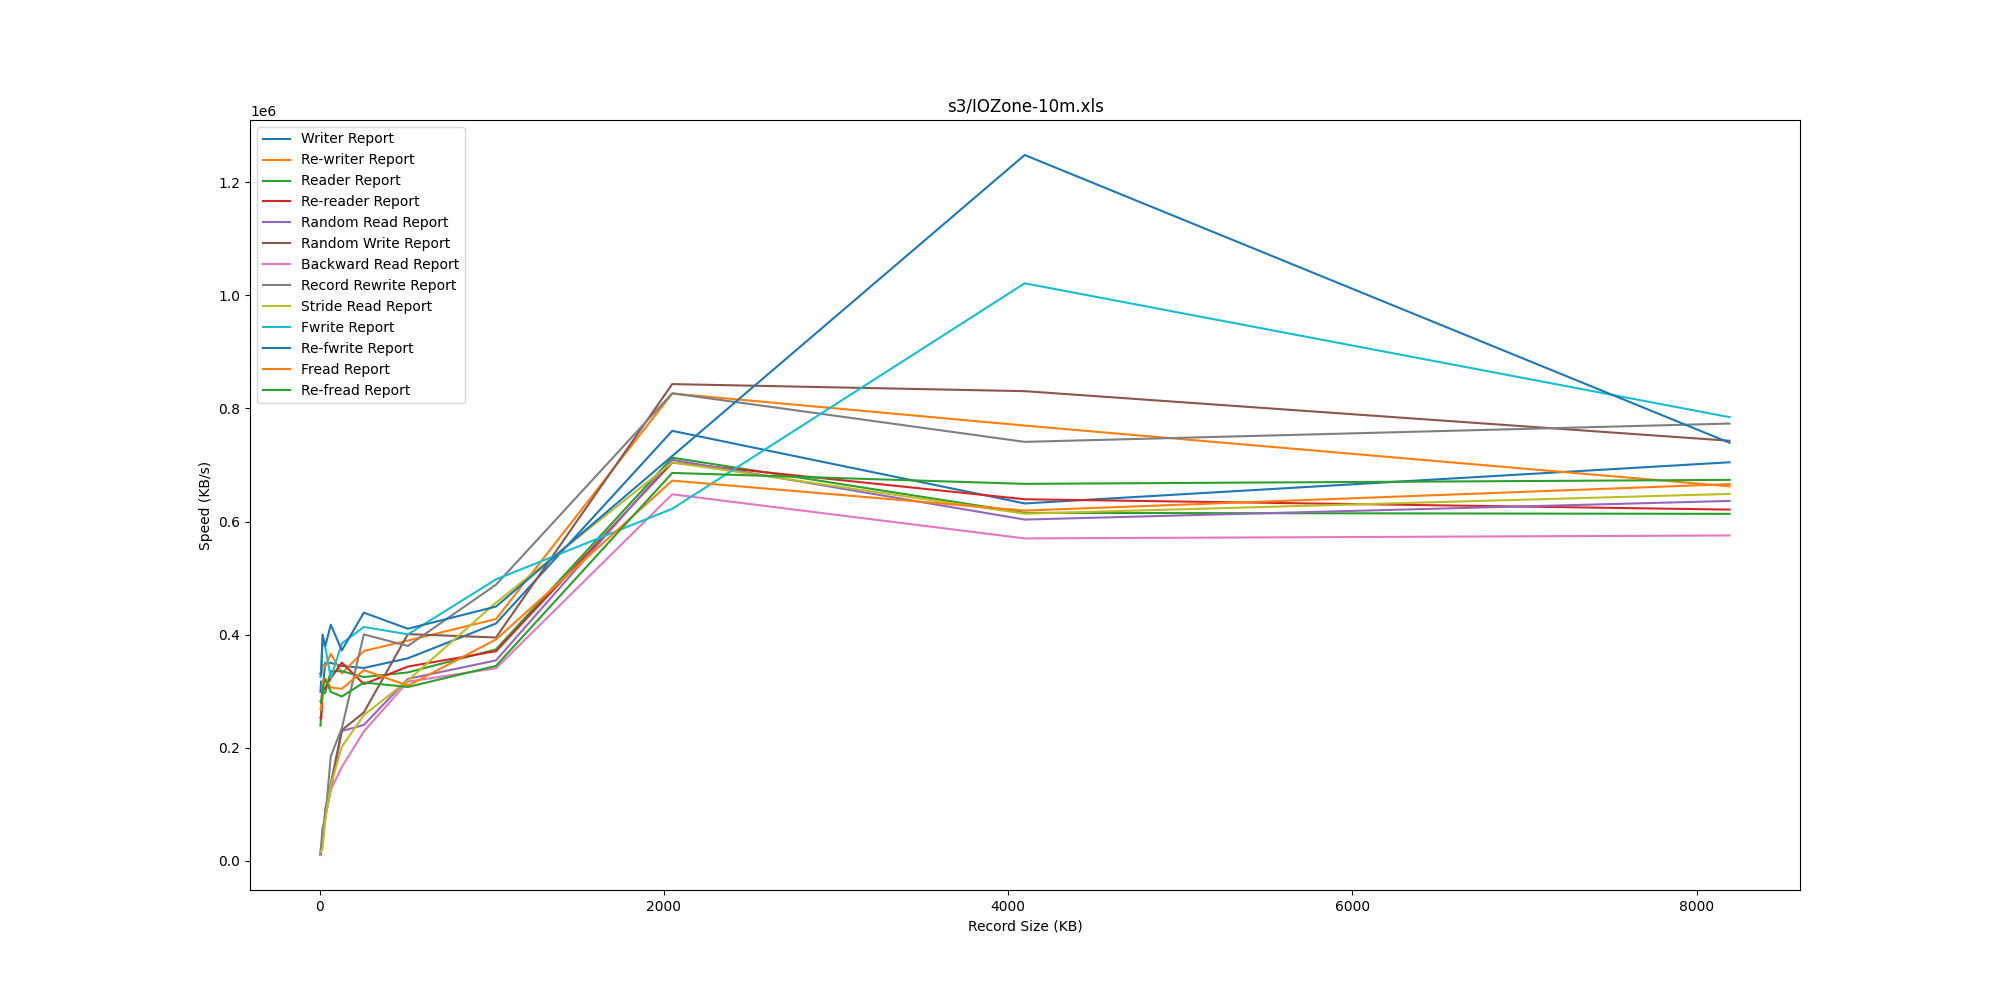
\includegraphics[width=\textwidth]{\baseimagedir/result/excel-to-chart/s3-IOZone-10m.xls.png}
    \caption{IOZone benchmark results for 10MB file in s3 directory}
    \label{fig:s3-10m}
\end{figure}

\begin{figure}
    \centering
    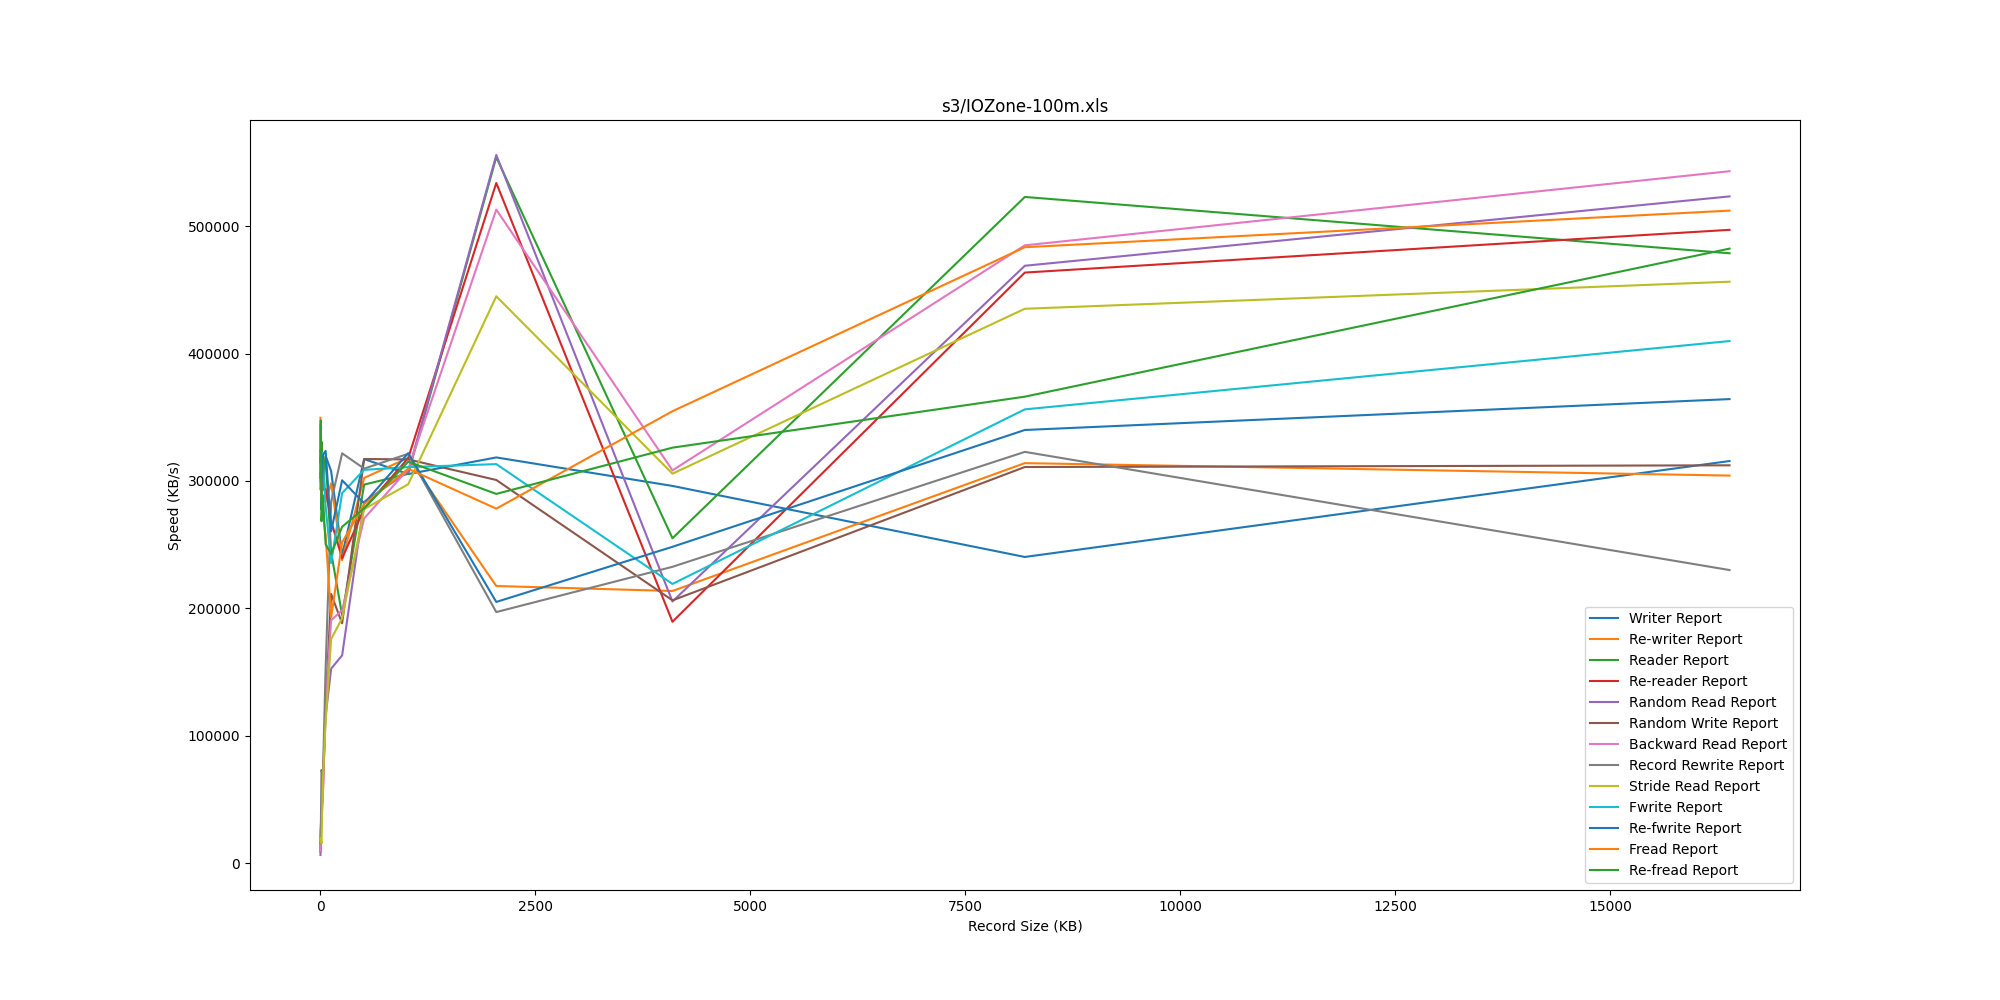
\includegraphics[width=\textwidth]{\baseimagedir/result/excel-to-chart/s3-IOZone-100m.xls.png}
    \caption{IOZone benchmark results for 100MB file in s3 directory}
    \label{fig:s3-100m}
\end{figure}

\begin{figure}
    \centering
    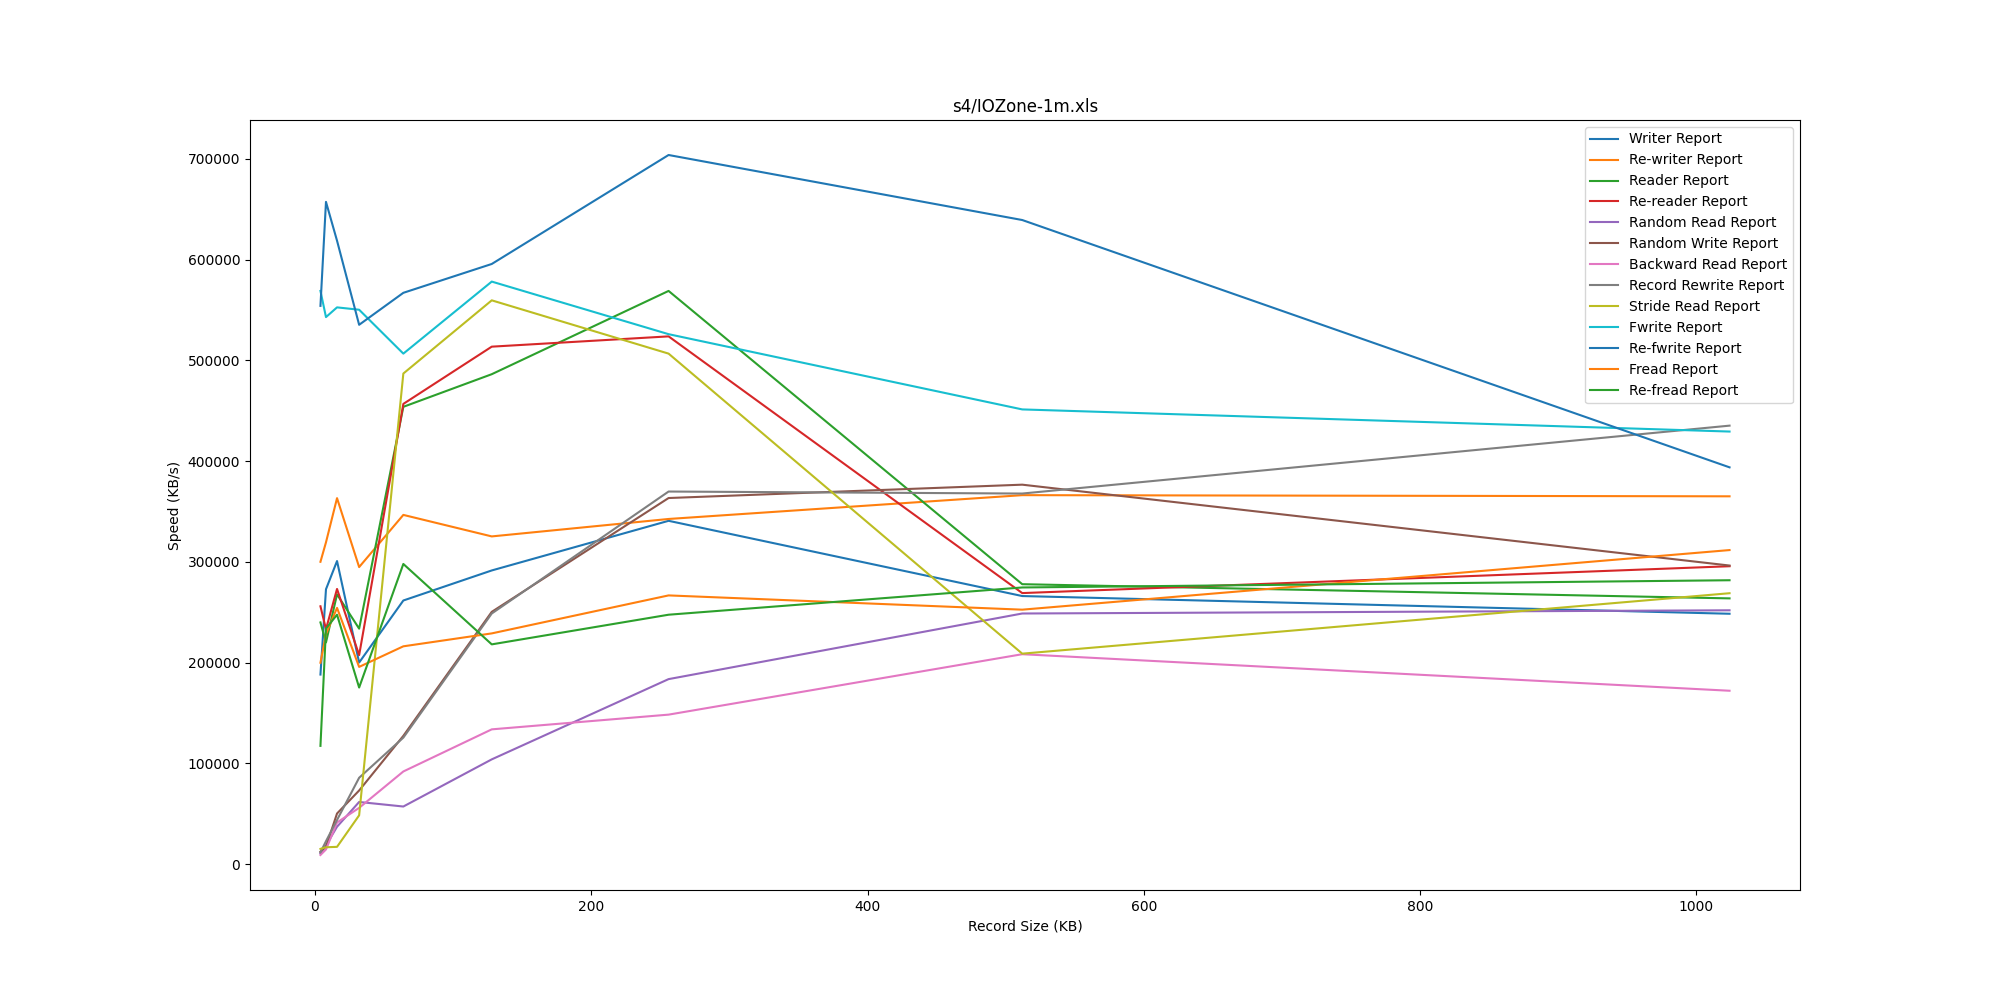
\includegraphics[width=\textwidth]{\baseimagedir/result/excel-to-chart/s4-IOZone-1m.xls.png}
    \caption{IOZone benchmark results for 1MB file in s4 directory}
    \label{fig:s4-1m}
\end{figure}

\begin{figure}
    \centering
    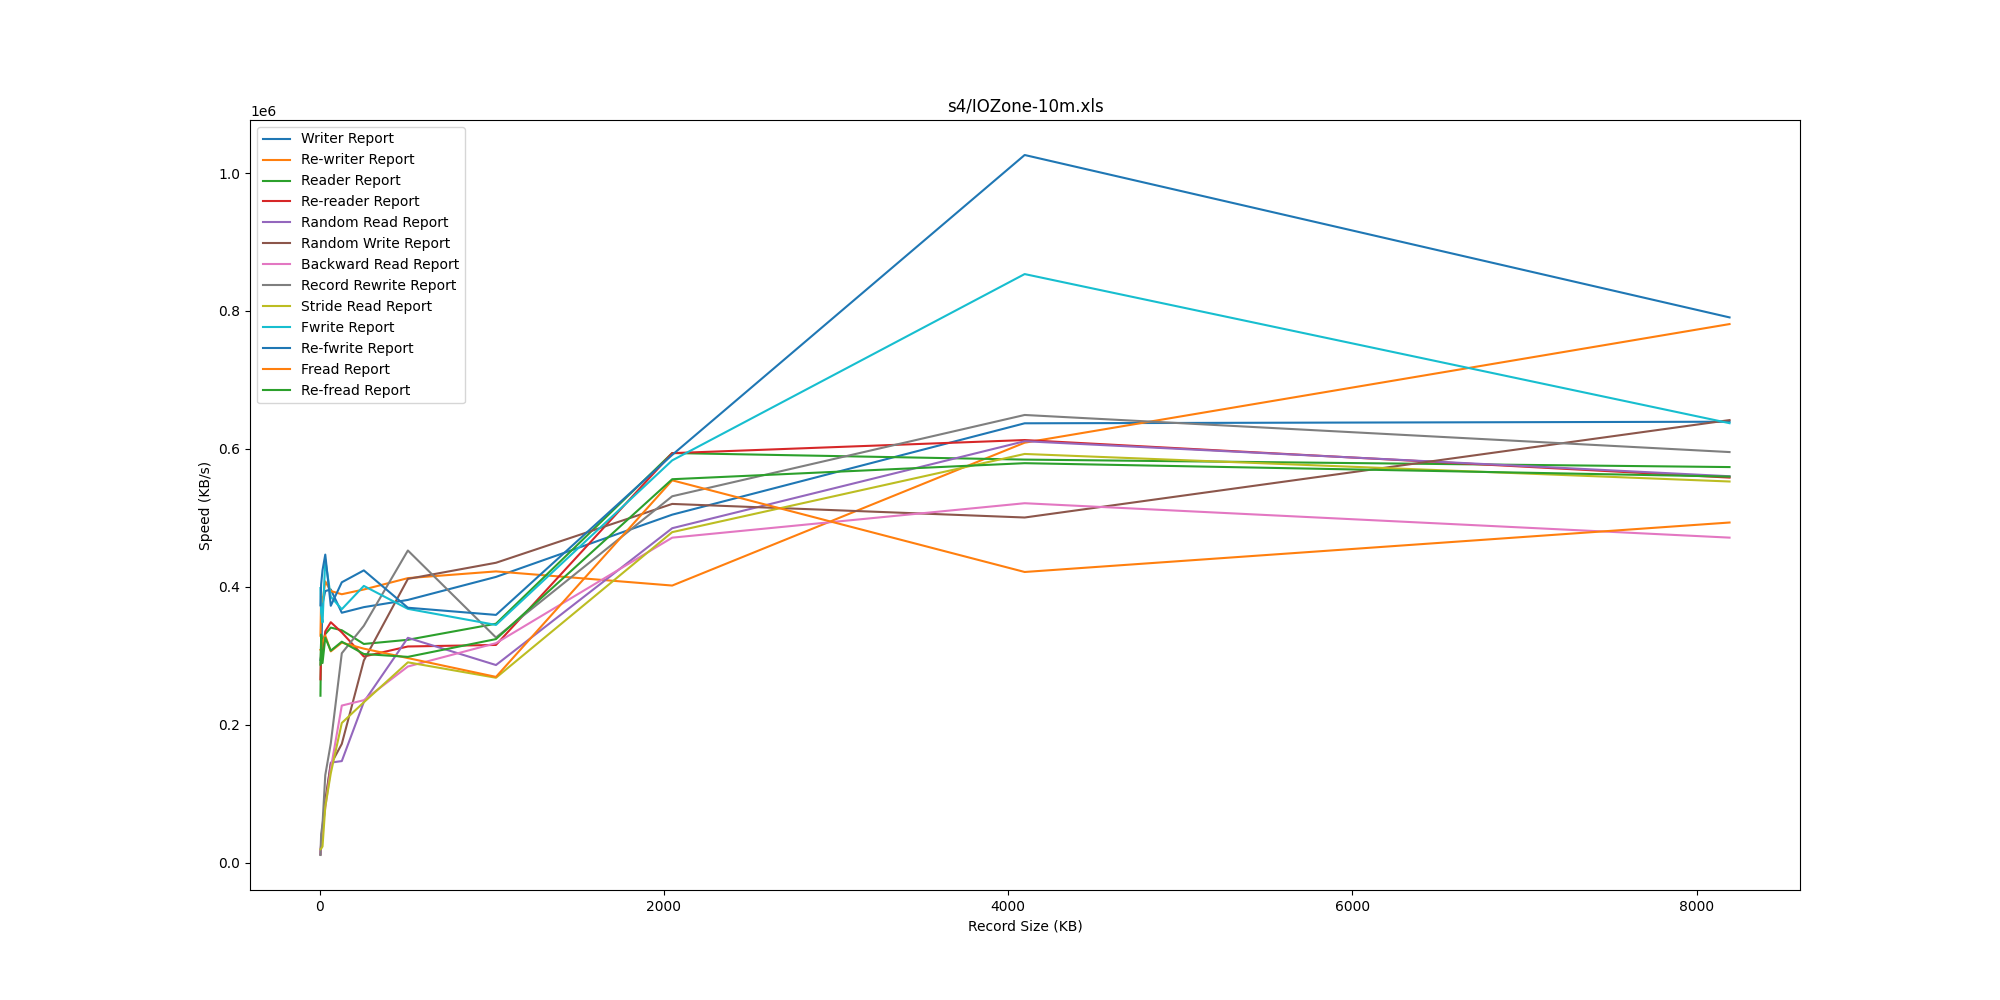
\includegraphics[width=\textwidth]{\baseimagedir/result/excel-to-chart/s4-IOZone-10m.xls.png}
    \caption{IOZone benchmark results for 10MB file in s4 directory}
    \label{fig:s4-10m}
\end{figure}

\begin{figure}
    \centering
    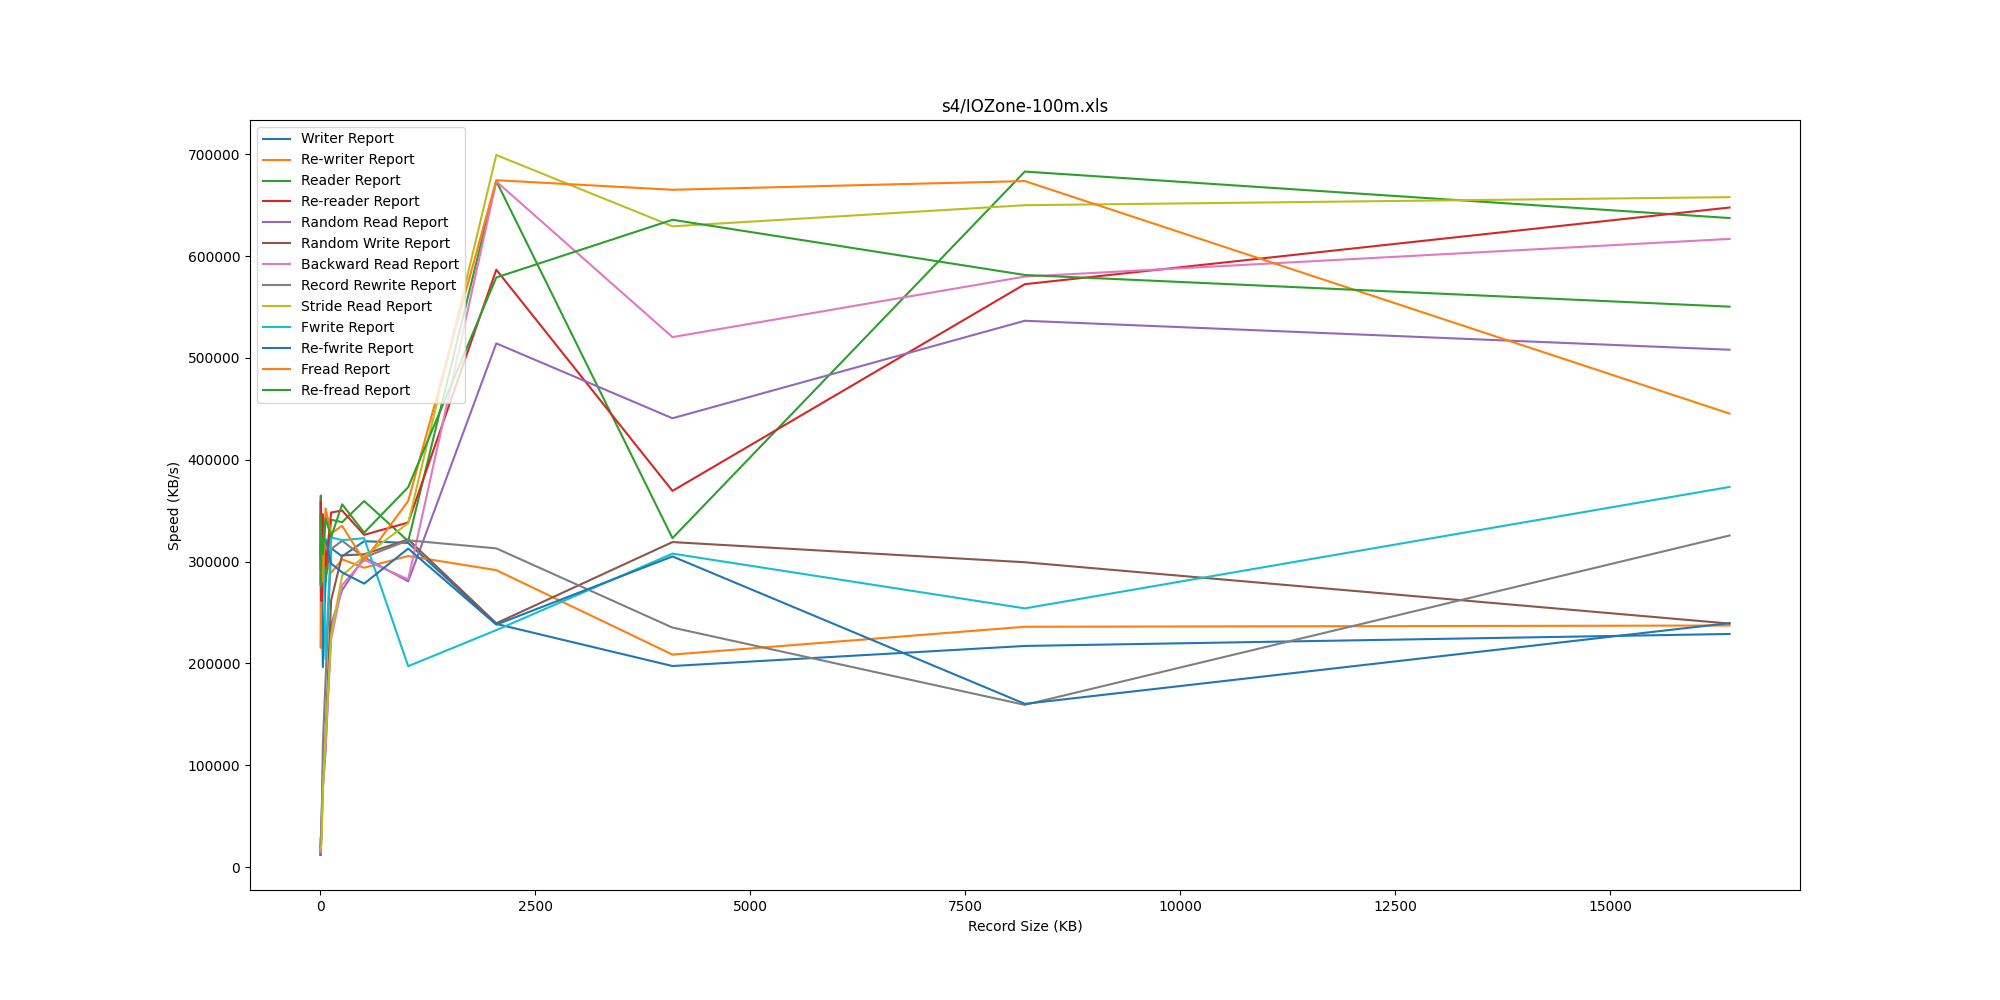
\includegraphics[width=\textwidth]{\baseimagedir/result/excel-to-chart/s4-IOZone-100m.xls.png}
    \caption{IOZone benchmark results for 100MB file in s4 directory}
    \label{fig:s4-100m}
\end{figure}

\section{Utilize BeeGFS Cache}
BeeGFS provides a mechanism for client-side caching. at the time of this research, BeeGFS provides support for two different caching scheme, buffered caching and native caching. Buffered caching provides a mechanism that results in higher streaming throughput compared to native caching, but it is limited by the cache size which is only few hundreds of kilo bytes. As for native caching scheme, BeeGFS client uses Linux's native page cache mechanism which can scale proportional to the size of the node's memory. In our experiment we used both scheme and conducted an experiment to evaluate the effects of BeeGFS client side caching on IO performance.

\subsection{Buffered Caching Results}

\seubsection{Native Caching Results}

\section{Utilize OpenCAS Cache}
%TODO parsa inja riz raje be behbud e performance toZh bede

\section{Conclusion}

\newpage
\printbibliography

\end{document}
